
\chapter{Erweiterte Regelungskonzepte auf Basis der exakten Linearisierung\label{chap:regler-varianten}}

Aufbauend auf den in Kapitel~\ref{chap:regler-grundlagen} entwickelten
Konzepten (relativer Grad und bestimmte Normalformen) lassen sich
etliche verschiedene Regler realisieren und damit auch unterschiedliche
regelungstechnische Aufgabenstellungen lösen~\cite{henson1997chap4}.
In diesem Kapitel werden verschiedene Regelungskonzepte, die auf der
exakten Linearisierung aufbauen, vorgestellt. Den nachfolgenden Betrachtungen
wird ein eingangsaffines Modell für die Regelstrecke zugrunde gelegt.
Während für theoretische Untersuchungen die Byrnes-Isidori-Normalform
bevorzugt wird, erfolgen praktische Berechnung oft mit der Eingangs-Ausgangs-Normalform.
Daher sind die vorgestellten Entwurfsverfahren auch leicht auf nicht
eingangsaffine Systeme zu übertragen.

\section{Trajektorienfolgeregelung mittels Rückführung (Feed\-back)\label{sec:Trajektorienfolgeregelung-Feedback}}

\subsection{Ausgangsfolgeregelung\label{subsec:Ausgangsfolgeregelung}}

Man betrachte eine eingangsaffine Regelstrecke der Form
\begin{equation}
\dot{x}=f(x)+g(x)u,\quad y=h(x)\label{eq:var-basissystem}
\end{equation}
mit glatten Vektorfeldern $f,g,:\mathcal{M}\to\R^{n}$ und einem glatten
Skalarfeld $h:\mathcal{M}\to\R$, wobei die Felder auf einer offenen
Menge $\mathcal{M}\subseteq\R^{n}$ definiert sind. Auf Basis der
Eingangs-Ausgangs-Linearisierung wird nachfolgend eine Ausgangsfolgeregelung
entworfen. Der Systemausgang~$y$ soll sich dabei asymp\-totisch
einem Referenzverlauf $y_{\text{ref}}:[0,\infty)\to\R$ annähern.
Die Darstellung beruht auf~\cite[Abschn.~{4.5}]{isidori3}.

System~(\ref{eq:var-basissystem}) habe einen wohldefinierten relativen
Grad $r\leq n$. Dann kann das System mit einer Zustandstransformation
$(\xi,\eta)=\Phi(x)$ in die Byrnes-Isidori-Normalform\index{Normalform!Byrnes-Isidori-}
\begin{equation}
\left.\begin{array}{lcl}
\dot{\xi}_{1} & = & \xi_{2}\\
 & \vdots\\
\dot{\xi}_{r-1} & = & \xi_{r}\\
\dot{\xi}_{r} & = & \alpha(\xi,\eta)+\beta(\xi,\eta)u\\
\dot{\eta}_{1} & = & q_{1}(\xi,\eta)\\
 & \vdots\\
\dot{\eta}_{n-r} & = & q_{n-r}(\xi,\eta)\\
y & = & \xi_{1}
\end{array}\right\} \quad\begin{array}{rcl}
\dot{\xi} & = & A\xi+b(\alpha(\xi,\eta)+\beta(\xi,\eta)u)\\
\dot{\eta} & = & q(\xi,\eta)\\
y & = & c^{T}\xi
\end{array}\label{eq:var-BI-NF}
\end{equation}
transformiert werden (siehe Abschnitt~\ref{subsec:Byrnes-Isidori-Normalform}).
Mit der Eingangs-Ausgangs-Linearisierung 
\begin{equation}
u=\frac{1}{\beta(\xi,\eta)}\left(v-\alpha(\xi,\eta)\right)=\frac{1}{L_{g}L_{f}^{r-1}h(x)}\left(v-L_{f}^{r}h(x)\right)\label{eq:var-linearisierung-FB}
\end{equation}
kompensiert man die im ersten Teilsystem von~(\ref{eq:var-BI-NF})
auftretenden Nichtlinearitäten derart, dass das Eingangs-Ausgangs-Verhalten
durch die Integratorkette
\begin{equation}
\left.\begin{array}{lcl}
\dot{\xi}_{1} & = & \xi_{2}\\
 & \vdots\\
\dot{\xi}_{r-1} & = & \xi_{r}\\
\dot{\xi}_{r} & = & v\\
y & = & \xi_{1}
\end{array}\right\} \quad\begin{array}{rcl}
\dot{\xi} & = & A\xi+bv\\
y & = & c^{T}\xi
\end{array}\label{eq:var-TS1-EA-linearisiert}
\end{equation}
beschrieben wird.

Zur Beschreibung des Folgeverhaltens wird der Fehler 
\begin{equation}
\varepsilon(t):=y(t)-y_{\text{ref}}(t)\quad\text{für}\quad t\geq0\label{eq:var-ausgangsfehler}
\end{equation}
als Differenz zwischen System- und Referenzausgang eingeführt. Für
den Zeitverlauf des Fehlers~$\varepsilon$ geben wir eine Fehlerdynamik
in Form einer linearen zeitinvarianten Differentialgleichung 
\begin{equation}
\varepsilon^{(r)}(t)+a_{r-1}\varepsilon^{(r-1)}(t)+\cdots+a_{1}\dot{\varepsilon}(t)+a_{0}\varepsilon(t)=0\label{eq:var-fehlerdynamik}
\end{equation}
der Ordnung~$r$ vor. Die Koeffizienten $a_{0},\ldots a_{r-1}\in\R$
sind dabei so zu wählen, dass das zu~(\ref{eq:var-fehlerdynamik})
gehörende charakteristische Polynom ein Hurwitz-Polynom ist. Dann
gilt 
\[
\lim_{t\to\infty}\varepsilon(t)\to0
\]
für alle Anfangswerte von~(\ref{eq:var-fehlerdynamik}), wodurch
das asymptotische Folgeverhalten gewährleistet ist.

Die gewünschte Fehlerdynmik~(\ref{eq:var-fehlerdynamik}) ist jetzt
noch in das System einzuprägen. Der vorgegebene Referenzverlauf $y_{\text{ref}}:[0,\infty)\to\R$
des Ausgangs sei $r$ mal stetig differenzierbar. Aus~(\ref{eq:var-ausgangsfehler})
folgt unmittelbar $\varepsilon^{(i)}(t)=y^{(i)}(t)-y_{\text{ref}}^{(i)}(t)$
für $i=0,\ldots,r$. Für die Integratorkette~(\ref{eq:var-TS1-EA-linearisiert})
ergibt sich daraus der Eingangsverlauf
\begin{equation}
\begin{array}{lcl}
v(t) & = & y^{(r)}(t)\\
 & = & y_{\text{ref}}^{(r)}(t)+\varepsilon^{(r)}(t)\\
 & = & y_{\text{ref}}^{(r)}(t)-a_{r-1}\varepsilon^{(r-1)}(t)-\cdots-a_{1}\dot{\varepsilon}(t)-a_{0}\varepsilon(t).
\end{array}\label{eq:var-PD-verallg}
\end{equation}
Ersetzt man die Zeitableitungen des Systemausgangs durch Lie-Ableitungen
$y^{(i)}(t)=L_{f}^{i}h(x(t))$ für $i=1,\ldots,r-1$ und bezieht die
linearisierende Zustandsrückführung~(\ref{eq:var-linearisierung-FB})
ein, so erhält man das Regelgesetz 
\begin{equation}
u=\frac{1}{L_{g}L_{f}^{r-1}h(x)}\left(y_{\text{ref}}^{(r)}(t)-L_{f}^{r}h(x)+\sum_{i=0}^{r-1}a_{i}\left(y_{\text{ref}}^{(i)}(t)-L_{f}^{i}h(x)\right)\right).\label{eq:folgeregelung-feedback}
\end{equation}
Dieses Regelgesetz kann man als Linearkombination 
\[
u=u_{\text{steuer}}+u_{\text{stab}}
\]
eines Anteils zur Vorsteuerung
\begin{equation}
u_{\text{steuer}}=\frac{1}{L_{g}L_{f}^{r-1}h(x)}\left(y_{\text{ref}}^{(r)}(t)-L_{f}^{r}h(x)\right)\label{eq:u-steuer-FB}
\end{equation}
und eines Anteils zur asymptotischen Stabilisierung 
\begin{equation}
u_{\text{stab}}=\frac{1}{L_{g}L_{f}^{r-1}h(x)}\sum_{i=0}^{r-1}a_{i}\left(y_{\text{ref}}^{(i)}(t)-L_{f}^{i}h(x)\right)\label{eq:u-stab-FB}
\end{equation}
auffassen. Man spricht dabei von einer \emph{Struktur mit zwei Freiheits\-graden}~\cite{horowitz1963synthesis,kreisselmeier1999}.
Der Steuerungsanteil~(\ref{eq:u-steuer-FB}) wird unter Verwendung
der Hirschorn-Inversen\index{Hirschorn-Inverse} entlang der Systemtrajektorie~$x$
gebildet (siehe Anmerkung~\ref{rem:Hirschorn-Inverse}). Ein Trajektoriengenerator
stellt die Referenztrajektorie bereit. Abb.~\ref{fig:Trajektorienfolgeregelung-FB}
verdeutlicht das Zusammenwirken der verschiedenen Anteile im geschlossenen
Regelkreis.

\begin{figure}
\begin{centering}
\resizebox{0.95\textwidth}{!}{\input{Traj_FB.pdftex_t}}
\par\end{centering}
\caption{Struktur der Trajektorienfolgeregelung mittels Rückführung\label{fig:Trajektorienfolgeregelung-FB}}

\end{figure}

\medskip{}

Durch die im Regelgesetz~(\ref{eq:folgeregelung-feedback}) auftretende
Referenztrajektorie $t\mapsto y_{\text{ref}}(t)$ ist das rückgeführte
System zeitvariant, so dass man die Stabilitätsaussagen aus den Sätzen~\ref{thm:Stabilisierung-EA-lokal}
oder~\ref{thm:Stabilisierung-EA-global} nicht unmittelbar übernehmen
kann. Allerdings lassen sich die Überlegungen von Satz~\ref{thm:Stabilisierung-EA-global-fuehrungssignal}
übertragen. Dazu betrachten wir das System~(\ref{eq:var-basissystem})
in der Byrnes-Isidori-Normalform~(\ref{eq:var-BI-NF}). Der Zustand~$\xi$
des ersten Teilsystems von~(\ref{eq:var-BI-NF}) ist durch den Ausgang
und seine Zeitableitungen gegeben:
\begin{equation}
\xi_{1}=y,\,\xi_{2}=\dot{y},\,\ldots,\,\xi_{r}=y^{(r-1)}.\label{eq:Zustand-xi-durch-y}
\end{equation}
Der Referenzzustand $\xi_{\text{ref}}$ lässt sich in gleicher Weise
durch $\xi_{1,\text{ref}}=y_{\text{ref}},\ldots,\xi_{r,\text{ref}}=y_{\text{ref}}^{(r-1)}$
beschreiben. Die Differenz $\tilde{\xi}=\xi-\xi_{\text{ref}}$ liefert
die Koordinaten des Fehlersystems mit $\tilde{\xi}_{1}=\varepsilon,\ldots,\tilde{\xi}_{r}=\varepsilon^{(r-1)}$.
Die Fehlerdynamik~(\ref{eq:var-fehlerdynamik}) lässt sich dann als
Zustandsraummodell
\begin{equation}
\left.\begin{array}{lcl}
\dot{\tilde{\xi}}_{1} & = & \tilde{\xi}_{2}\\
 & \vdots\\
\dot{\tilde{\xi}}_{r-1} & = & \tilde{\xi}_{r}\\
\dot{\tilde{\xi}}_{r} & = & -a_{0}\tilde{\xi}_{1}-\cdots-a_{r-1}\tilde{\xi}_{r}
\end{array}\right\} \quad\dot{\tilde{\xi}}=(A-bk^{T})\,\tilde{\xi}\label{eq:folgesystem-FB1}
\end{equation}
mit $k=(a_{0},\ldots,a_{r-1})^{T}$ angeben. Mit $\xi=\xi_{\text{ref}}+\tilde{\xi}$
ergibt sich für das zweite Teilsystem die Form
\begin{equation}
\dot{\eta}=q(\xi_{\text{ref}}+\tilde{\xi},\eta).\label{eq:folgesystem-FB2}
\end{equation}

Nach diesen Vorüberlegungen kann folgende Aussage getroffen werden:
\begin{theorem}
\label{thm:Stabilisierung-FB}Das System~(\ref{eq:var-basissystem})
habe den Arbeitspunkt $p\in\mathcal{M}$ (für $u=0$) und den gleichmäßigen
relativen Grad $r<n$. Zusätzlich sei das System global rück\-führ\-äquivalent
zu der Form~(\ref{eq:var-BI-NF}) mit der Ruhelage $(\xi,\eta)=(0,0)$.
Die Reglerverstärkung $k\in\R^{r}$ sei so gewählt, dass das zur Fehlerdynamik~(\ref{eq:var-fehlerdynamik})
gehörende charakteristische Polynom ein Hurwitz-Polynom ist. Zusätzlich
sei der Referenzverlauf~$y_{\text{ref}}$ bis zur Ableitungsordnung
$r-1$ beschränkt, d.\,h. es gibt eine Schranke $M>0$, so dass
\begin{equation}
\left|y_{\text{ref}}^{(i)}(t)\right|<M\label{eq:yref-beschraenkt-in-Cr}
\end{equation}
für alle $t\geq0$ und $i=0,\ldots,r-1$. Ist das System stark minimalphasig,
dann bleiben die Systemtrajektorien beschränkt.
\end{theorem}
\begin{svmultproof2}
Da globale Rückführäquivalenz zur Form~(\ref{eq:var-BI-NF}) angenommen
wird, kann die Stabilitätsbetrachtung auf Basis der Gln.~(\ref{eq:folgesystem-FB1})
und~(\ref{eq:folgesystem-FB2}) erfolgen. Weil alle Eigenwerte der
Matrix $A-bk^{^{T}}$nach Wahl der Reglerverstärkung~$k$ negative
Realteile besitzen, klingt~$\tilde{\xi}$ ab, d.\,h. $\tilde{\xi}(t)\to0$
für $t\to\infty$. Damit ist~$\tilde{\xi}$ beschränkt. Mit Gl.~(\ref{eq:yref-beschraenkt-in-Cr})
ist~$\xi_{\text{ref}}$ und damit die auch Summe $\xi_{\text{ref}}+\tilde{\xi}$
beschränkt. Mit der angenommenen starken Minimalphasigkeit ist das
zweite Teilsystem~(\ref{eq:folgesystem-FB2}) eingangs-zustands-stabil,
so dass $\eta$ beschränkt bleibt. Da die Transformation ein globaler
Diffeomorphismus ist, bleibt auch die System\-trajektorie~$x$ beschränkt.
\end{svmultproof2}

Für $r=n$ tritt das zweites Teilsystem~(\ref{eq:folgesystem-FB2})
nicht auf. In diesem Fall erhält man durch~(\ref{eq:folgesystem-FB1})
insgesamt eine lineare zeitinvariante Fehlerdynamik.

\medskip{}

Die dargelegten Überlegungen lassen sich unmittelbar auf Mehr\-größen\-systeme
übertragen. Die Kompensation der Nichtlinearitäten erfolgt simultan
mit der Entkopplung der Teilsysteme (siehe Abschnitt~\ref{sec:Mehrvariable-Systeme}).
Die Trajektorienfolgeregelung wird dann für jeden einzelnen Ausgang
in der beschriebenen Weise durchgeführt. Bei einem vollständig aktuierten
mechanischen System lässt sich die Trajektorienfolgeregelung besonders
einfach gestalten: 
\begin{remark}
\label{rem:Mechanisches-System-Feedback}Wir betrachten ein mechanisches
System, welches durch eine Bewegungsgleichung der Form 
\begin{equation}
M(q)\ddot{q}+C(q,\dot{q})=\tau\label{eq:mani-euler-lagrange-tracking}
\end{equation}
mit den verallgemeinerten Positionen~$q$, den verallgemeinerten
Geschwindigkeiten~$\dot{q}$ und der Massenmatrix $M(q)$ beschrieben
wird. Der Vektor~$\tau$ enthält die eingeprägten Kräfte bzw. Momente
und der Vektor $C(q,\dot{q})$ alle weiteren Kräfte. Die Forderung
\[
\ddot{q}\stackrel{!}{=}v
\]
einer exakten Kompensation der Nichtlinearitäten führt zunächst auf
das (linearisierende) Stellgesetz
\begin{equation}
\tau=M(q)\,v+C(q,\dot{q}),\label{eq:mech-linearisierung-feedback}
\end{equation}
vgl. Anmerkung~\ref{rem:Mechanisch-relativer-grad}. Die Stabilisierung
entlang einer zweimal stetig differenzierbaren Referenztrajektorie~$q_{\text{ref}}$
erfolgt durch die als PD-Regler\index{PD-Regler} interpretierbare
Rückführung
\begin{equation}
v=\ddot{q}_{\text{ref}}+K_{D}\left(\dot{q}_{\text{ref}}-\dot{q}\right)+K_{P}\left(q_{\text{ref}}-q\right)\label{eq:mech-stabiliserung}
\end{equation}
mit passenden Diagonalmatrizen~$K_{P}$ und~$K_{D}$. Setzt man
das daraus resultierende Stellgesetz 
\begin{equation}
\tau=M(q)\cdot\left[\ddot{q}_{\text{ref}}+K_{D}\left(\dot{q}_{\text{ref}}-\dot{q}\right)+K_{P}\left(q_{\text{ref}}-q\right)\right]+C(q,\dot{q})\label{eq:tau-mech-FB}
\end{equation}
in die Bewegungsgleichung~(\ref{eq:mani-euler-lagrange-tracking})
ein, so erhält man eine exakt lineare zeit\-invariante Fehlerdynamik
\[
0=\ddot{q}_{\text{ref}}-\ddot{q}+K_{D}\left(\dot{q}_{\text{ref}}-\dot{q}\right)+K_{P}\left(q_{\text{ref}}-q\right).
\]
Bei diesem Ansatz nutzt man die Bewegungsgleichung zur Berechnung
der einzuprägenden Momente. Man spricht daher von der \emph{Methode
der berechneten Momente} (engl. \emph{computed torque method}).
\end{remark}

\begin{remark}
\label{rem:PI-Feedback}PI- und PID-Regler sind in der industriellen
Praxis die am häufigsten eingesetzten Reglertypen~\cite{marlin2000,odwyer2009handbook}.
Mit dem I-Anteil lassen sich bleibende Regelabweichungen kompensieren
und Störungen unterdrücken~\cite{datta2000}. Die Rückführung~(\ref{eq:folgeregelung-feedback})
kann man unter Bezug auf Gl.~(\ref{eq:var-PD-verallg}) als verallgemeinerten
PD-Regler\index{PD-Regler} auffassen. Zur Ergänzung eines I-Anteils
erweitert man die Fehlerdynamik~(\ref{eq:var-fehlerdynamik}) zu
\[
\varepsilon^{(r)}(t)+a_{r-1}\varepsilon^{(r-1)}(t)+\cdots+a_{1}\dot{\varepsilon}(t)+a_{0}\varepsilon(t)+a_{I}\int_{0}^{t}\varepsilon(\tau)\d\tau=0
\]
mit dem zusätzlichen Koeffizienten $a_{I}>0$. Der I-Anteil wird dabei
nach der Kompensation der Nichtlinearitäten durch~(\ref{eq:var-linearisierung-FB})
eingefügt. In den Originalkoordinaten erhält man daraus die Zustandsrückführung
\[
u=\frac{1}{L_{g}L_{f}^{r-1}h(x)}\left(a_{I}\!\int_{0}^{t}\!\left(y_{\text{ref}}(\tau)-h(x(\tau))\right)\d\tau+\sum_{i=0}^{r}a_{i}\left(y_{\text{ref}}^{(i)}(t)-L_{f}^{i}h(x)\right)\right)
\]
mit $a_{r}:=1$, vgl.~\cite{kravaris1987,henson1991critique}. Diese
Rückführung lässt sich als verallgemeinerter PID-Regler\index{PID-Regler}
interpretieren~\cite{sira-ramirez2002gpid}. Alternativ kann man
dem (nicht eingangs-ausgangs-linearisierten) Originalsystem auch einen
Integrator vorschalten~\cite{mahout2003}. Das erweiterte System
hat dann den relativen Grad $r+1$ (vgl. Abschnitt~\ref{subsec:Relativer-Grad-nichtaffine})
und kann mit der hinsichtlich~$r$ entsprechend an\-ge\-passten
Rückführung~(\ref{eq:folgeregelung-feedback}) geregelt werden.
\end{remark}

\subsection{Überführung zwischen Ruhelagen\label{subsec:Ueberfuehrung-zwischen-Ruhelagen}}

Eine besonders praxisrelevante Aufgabenstellung im Rahmen der Trajektorienfolgeregelung
ist die Überführung des Systems von einer Ruhelage $x^{0}\in\mathcal{M}$
in eine andere Ruhelage $x^{1}\in\mathcal{M}$. Hinsichtlich des Ausgangs
bedeutet das einen Übergang von $y^{0}=h(x^{0})$ zu $y^{1}=h(x^{1})$.
Gesucht ist ein Referenzverlauf $y_{\text{ref}}:[0,T]\to\R$ des Ausgangs,
so dass die Ruhelage $x^{0}=x(0)$ in die Ruhelage $x^{1}=x(T)$ überführt
wird (siehe Abb.~\ref{fig:Referenztrajektorie-Ausgang}). Die Ruhelagenüberführung
erfolgt in diesem Abschnitt für das durch Rückführung linearisierte
erste Teil\-system~(\ref{eq:var-TS1-EA-linearisiert}). Die Überführung
des Zustands~$x$ bzw. $(\xi,\eta)$ des Gesamtsystems wird in Abschnitt~\ref{sec:Trajektorienfolgeregelung-Feedforward}
behandelt. 
\begin{figure}
\begin{centering}
\resizebox{0.7\textwidth}{!}{\input{Ruhelagenueberfuehrung.pdftex_t}}
\par\end{centering}
\caption{Referenztrajektorie des Ausgangs bei einer Ruhelagenüberführung\label{fig:Referenztrajektorie-Ausgang}}
\end{figure}

Der Zustand~$\xi$ des Systems~(\ref{eq:var-TS1-EA-linearisiert})
lässt sich durch den Ausgang und seine Zeitableitungen erfassen, vgl.
Gl.~(\ref{eq:Zustand-xi-durch-y}). Die Ruhelagen vor und nach dem
Überführungsvorgang sind daher durch die $2r$ Randbedingungen
\begin{equation}
\begin{array}{llll}
y_{\text{ref}}(0)=y^{0}, & \dot{y}_{\text{ref}}(0)=0, & \ldots, & y_{\text{ref}}^{(r-1)}(0)=0\\
y_{\text{ref}}(T)=y^{1}, & \dot{y}_{\text{ref}}(T)=0, & \ldots, & y_{\text{ref}}^{(r-1)}(T)=0
\end{array}\label{eq:var-randbedingungungen1}
\end{equation}
eindeutig festgelegt. Wählt man für die Überführung zwischen den Ruhelagen
einen hinreichend glatten Verlauf des Referenzausgangs $y_{\text{ref}}:[0,T]\to\R$,
so dass diese Randbedingungen erfüllt sind, dann erhält man damit
auch einen stetigen Übergang des Zustands~$\xi$. Fordert man zusätzlich
\begin{equation}
y_{\text{ref}}^{(r)}(0)=y_{\text{ref}}^{(r)}(T)=0,\label{eq:var-randbedingungungen2}
\end{equation}
dann ist wegen der letzten Differentialgleichung von~(\ref{eq:var-TS1-EA-linearisiert})
auch der für die Überführung benötigte Eingangsverlauf stetig. Mit
den Gln.~(\ref{eq:var-randbedingungungen1}) und~(\ref{eq:var-randbedingungungen2})
ergeben sich insgesamt $2r+2$ Randbedingungen, die der gesuchte Referenzverlauf
$y_{\text{ref}}$ des Ausgangs erfüllen soll.

Für den Übergang von $y^{0}=y_{\text{ref}}(0)$ zu $y^{1}=y_{\text{ref}}(T)$
unter Beachtung der o.\,g. Randbedingungen könnte man aus einer großen
Menge möglicher Ansatzfunktionen wählen (z.\,B. Splines oder Linearkombinationen
trigonometrischer Funktionen). Ein besonders einfacher Ansatz ist
durch ein Polynom gegeben. Um nicht in jedem Einzelfall das benötigte
Polynom erneut auszurechnen bietet es sich an, ein normiertes Polynom~$\sigma$
zu bestimmen, welches von $\sigma(0)=0$ auf $\sigma(1)=1$ unter
Berücksichtigung der entsprechenden Randbedingungen in den Ableitungen
übergeht. Für $2r+2$ Parameter muss das Polynom~$\sigma$ mindestens
mit dem Grad $2r+1$ angesetzt werden.
\begin{example}
\label{exa:normiertes-uebergangspolynom}Für $r=1$ würde man ein
Polynom von Grad $2r+1=3$ ansetzen:
\[
\sigma(t)=\sigma_{0}+\sigma_{1}t+\sigma_{2}t^{2}+\sigma_{3}t^{3}.
\]
Die Parameter~$\sigma_{0}$ und~$\sigma_{1}$ erhält man aus den
Bedingungen am linken Rand:
\[
\begin{array}{lclcl}
\sigma(0) & = & \sigma_{0} & \stackrel{!}{=} & 0,\\
\dot{\sigma}(0) & = & \sigma_{1} & \stackrel{!}{=} & 0.
\end{array}
\]
Die Bedingungen am rechten Rand 
\[
\left.\begin{array}{lclcl}
\sigma(1) & = & \sigma_{2}+\sigma_{3} & \stackrel{!}{=} & 1\\
\dot{\sigma}(1) & = & 2\sigma_{2}+3\sigma_{3} & \stackrel{!}{=} & 0
\end{array}\right\} \quad\Leftrightarrow\quad\left(\begin{array}{cc}
1 & 1\\
2 & 3
\end{array}\right)\left(\begin{array}{c}
\sigma_{2}\\
\sigma_{3}
\end{array}\right)=\left(\begin{array}{c}
1\\
0
\end{array}\right)
\]
liefern $\sigma_{2}=3$ und $\sigma_{3}=-2$ und damit $\sigma(t)=3t^{2}-2t^{3}$. 

\end{example}
Der in Beispiel~\ref{exa:normiertes-uebergangspolynom} beschriebene
Ansatz führt bei polynomialen Ansatzfunktionen immer auf ein lineares
Gleichungssystem. Allerdings können die gesuchten Übergangspolynome
auch über eine direkte Formel berechnet werden~\cite{piazzi2001tac,piazzi2001automatica}:
\begin{equation}
\sigma(t)=\frac{(2r+1)!}{r!}\sum_{i=r+1}^{2r+1}\frac{(-1)^{i-r-1}}{(i-r-1)!\,(2r+1-i)!\cdot i}\,t^{i}.\label{eq:formel-uebergangspolynom}
\end{equation}
Basierend auf dem normierten Übergangspolynom~$\sigma$ lässt sich
jetzt der Übergang von $y^{0}=y_{\text{ref}}(0)$ zu $y^{1}=y_{\text{ref}}(T)$
durch die abschnittsweise definierte Funktion
\begin{equation}
y_{\text{ref}}(t)=\left\{ \begin{array}{ccl}
y^{0} &  & t<0\\
y^{0}+(y^{1}-y^{0})\cdot\sigma\left(\frac{t}{T}\right) & \quad\text{für}\quad & 0\leq t\leq T\\
y^{1} &  & t>T
\end{array}\right.\label{eq:yref-allgemein}
\end{equation}
spezifizieren (vgl. Abb.~\ref{fig:Referenztrajektorie-Ausgang}).

\begin{example}
\label{exa:hochsetzsteller-folgeregelung-feedback}Man betrachte das
gemittelte Modell des Hochsetzstellers\index{Hochsetzsteller} aus
Abschnitt~\ref{subsec:Hochsetzsteller} mit den dort angegebenen
Parameterwerten:
\begin{equation}
\begin{array}{lcl}
\dot{x}_{1} & = & -(1-u)\frac{1}{L}x_{2}+\frac{E}{L},\\
\dot{x}_{2} & = & (1-u)\frac{1}{C}x_{1}-\frac{1}{RC}x_{2}.
\end{array}\label{eq:var-hochsetzsteller}
\end{equation}
Gewünscht ist ein Übergang der Ausgangsspannung von $20\,\text{V}$
auf $25\,\text{V}$ in einem Zeitintervall der Länge $T=50\,\text{ms}$.

Verwendet man für den Reglerentwurf den Strom\footnote{Aus Anwendungssicht wäre es wünschenswert, die Spannung direkt als
Referenzgröße nutzen zu können. Mit dem hier beschriebenen Zugang
ist das leider nicht möglich, da die zugehörige Nulldynamik instabil
ist (vgl. Abschnitt~\ref{subsec:Hochsetzsteller-Ausgang-Spannung}).} als Ausgang
\begin{equation}
y=h(x)=x_{1},\label{eq:hochsetzsteller-ausgang-strom-tracking}
\end{equation}
so hat das System den relativen Grad $r=1$. Damit lässt sich das
normierte Übergangspolynom $\sigma(t)=3t^{2}-2t^{3}$ aus Beispiel~\ref{exa:normiertes-uebergangspolynom}
nutzen. Der Übergang zwischen den o.\,g. Spannungen entspricht einem
Übergang des Stroms von $y^{0}=x_{1}(0)=2,\bar{6}\,\text{\text{A}}$
auf $y^{1}=x_{1}(T)=4,1\bar{6}\,\text{A}$. Auf Basis des sich daraus
ergebenden Referenzverlaufs
\begin{equation}
y_{\text{ref}}(t)=\frac{8}{3}+1800t^{2}-24000t^{3}\label{eq:hochsetzsteller-yref-strom}
\end{equation}
nach Gl.~(\ref{eq:yref-allgemein}) mit $t$ in~$\text{s}$ und~$y_{\text{ref}}$
in~$\text{A}$ nimmt das Regelgesetz~(\ref{eq:folgeregelung-feedback})
die Form
\end{example}
\begin{eqnarray*}
u & = & \frac{1}{L_{g}h(x)}\left(\dot{y}_{\text{ref}}(t)-L_{f}h(x)+a_{0}(y_{\text{ref}}(t)-h(x))\right)\\
 & = & \frac{L}{x_{2}}\left(\dot{y}_{\text{ref}}(t)-\frac{E-x_{2}}{L}+a_{0}(y_{\text{ref}}(t)-x_{1})\right)
\end{eqnarray*}
mit einem Koeffizienten $a_{0}>0$ an.

Verwendet man alternativ die elektrische Energie als Ausgang 
\begin{equation}
y=h(x)=\frac{L}{2}x_{1}^{2}+\frac{C}{2}x_{2}^{2},\label{eq:hochsetzsteller-ausgang-energie-tracking}
\end{equation}
so hat das System den relativen Grad $r=2$, d.\,h. man führt eine
Eingangs-Zustands-Linearisierung durch. Aus Gl.~(\ref{eq:formel-uebergangspolynom})
erhält man das Übergangspolynom $\sigma(t)=10t^{3}-15t^{4}+6t^{5}$.
Für~(\ref{eq:hochsetzsteller-ausgang-energie-tracking}) wird der
Übergang von $y^{0}=0,201\bar{7}\,\text{Ws}$ auf $y^{1}=0,3168402\bar{7}\,\text{Ws}$
entsprechend Gl.~(\ref{eq:yref-allgemein}) geplant 
\begin{equation}
y_{\text{ref}}(t)=0,201\bar{7}+9205t^{3}-276150t^{4}+2209200t^{5},\label{eq:hochsetzsteller-yref-energie}
\end{equation}
wobei $t$ in~$\text{s}$ und $y_{\text{ref}}$ in~$\text{Ws}$
angegeben sind. Das Regelgesetz hat die Gestalt 
\[
u=\frac{1}{L_{g}L_{f}h(x)}\left(\ddot{y}_{\text{ref}}(t)\!-\!L_{f}^{2}h(x)+a_{1}((\dot{y}_{\text{ref}}(t)\!-\!L_{f}h(x)))+a_{0}(y_{\text{ref}}(t)\!-\!h(x))\right)
\]
mit den Lie-Ableitungen aus Gl.~(\ref{eq:Hochsetzsteller-Lie-Ableitungen-Energie})
und den Koeffizienten $a_{0},a_{1}>0$ (Stodola-Bedingung).

Abb.~\ref{fig:Hochsetzsteller-Tracking} zeigt die numerischen Ergebnisse
für beide Fälle ($r=1$ bzw. $r=2$ für Eingangs-Ausgangs- bzw. Eingangs-Zustands-Linearisierung).
Die Koeffizienten $a_{0},a_{1}$ der Reglerverstärkung wurden entsprechend
Abschnitt~\ref{subsec:Hochsetzsteller} gewählt. Mit der Eingangs-Zustands-Linearisierung
ist ein schnelleres Einschwingen möglich. Allerdings weist der Strom
in diesem Fall auch ein leichtes Überschwingen auf (Abb.~\ref{fig:Hochsetzsteller-Tracking}
oben).

\begin{figure}
\begin{centering}
\includegraphics[width=0.8\textwidth]{Hochsetzsteller_Tracking_FB}
\par\end{centering}
\caption{Referenztrajektorien bzw. Simulation des ungestörten Hochsetzstellers\label{fig:Hochsetzsteller-Tracking}}
\end{figure}


\section{Trajektorienfolgeregelung mittels Aufschaltung (Feed\-forward)\label{sec:Trajektorienfolgeregelung-Feedforward}}

\subsection{Folgeregelung entlang einer bekannten Referenztrajektorie}

Wir widmen uns weiterhin dem Problem der Trajektorienfolgeregelung
und betrachten die in~\cite{hagenmeyer2003lncis,hagenmeyer2003}\nocite{zinober2003}
vorgestellten Lösungsansätze. Dabei gehen wir jetzt von einem bekannten
Referenzverlauf $x_{\text{ref}}:[0,T]\to\mathcal{M}$ des Zustands
aus. Befindet sich der Zustand des Systems~(\ref{eq:var-basissystem})
bereits auf der Referenztrajektorie, d.\,h. $x=x_{\text{ref}}$,
dann kann die in Gl.~(\ref{eq:var-linearisierung-FB}) durchgeführte
Kompensation der Nichtlinearitäten des ersten Teilsystems von~(\ref{eq:var-BI-NF})
auch auf Basis des Referenzzustands mit $(\xi_{\text{ref}},\eta_{\text{ref}})=\Phi(x_{\text{ref}})$
erfolgen: 
\begin{equation}
u=\frac{1}{\beta(\xi_{\text{ref}},\eta_{\text{ref}})}\left(v-\alpha(\xi_{\text{ref}},\eta_{\text{ref}})\right)=\frac{1}{L_{g}L_{f}^{r-1}h(x_{\text{ref}})}\left(v-L_{f}^{r}h(x_{\text{ref}})\right).\label{eq:var-linearisierung-FF}
\end{equation}
Zusammen mit der aus der vorgegebenen Fehlerdynamik~(\ref{eq:var-fehlerdynamik})
hergeleiteten Rückführung~(\ref{eq:folgeregelung-feedback}) erhält
man insgesamt das Regelgesetz 
\begin{equation}
u=\frac{1}{L_{g}L_{f}^{r-1}h(x_{\text{ref}}(t))}\left(y_{\text{ref}}^{(r)}(t)-L_{f}^{r}h(x_{\text{ref}}(t))+\sum_{i=0}^{r-1}a_{i}\left(y_{\text{ref}}^{(i)}(t)-L_{f}^{i}h(x)\right)\right).\label{eq:folgeregelung-feedforward}
\end{equation}
Der Unterschied zu dem Regelgesetz~(\ref{eq:folgeregelung-feedback})
besteht lediglich darin, dass die höchsten Lie-Ableitungen $L_{f}^{r}h(x)$
und $L_{g}L_{f}^{r-1}h(x)$ entlang der Referenztrajektorie~$x_{\text{ref}}$
anstelle der Systemtrajektorie~$x$ ausgewertet werden. Bei diesem
Zugang erwartet man im Vergleich zur Trajektorienfolgeregelung~(\ref{eq:folgeregelung-feedback})
mittels Rückführung eine größere Robustheit gegenüber Modellunbestimmtheiten.

Auch bei Gl.~(\ref{eq:folgeregelung-feedforward}) ist eine Aufspaltung
\begin{equation}
u=u_{\text{ref}}+u_{\text{stab}}\label{eq:u-aufspaltung-FF}
\end{equation}
in einen Anteil der Vorsteuerung
\begin{equation}
u_{\text{ref}}=\frac{1}{L_{g}L_{f}^{r-1}h(x_{\text{ref}}(t))}\left(y_{\text{ref}}^{(r)}(t)-L_{f}^{r}h(x_{\text{ref}}(t))\right)\label{eq:u-steuer-FF}
\end{equation}
und einen Anteil zur asymptotischen Stabilisierung
\begin{equation}
u_{\text{stab}}=\frac{1}{L_{g}L_{f}^{r-1}h(x_{\text{ref}}(t))}\sum_{i=0}^{r-1}a_{i}\left(y_{\text{ref}}^{(i)}(t)-L_{f}^{i}h(x)\right)\label{eq:u-stab-FF}
\end{equation}
möglich. Die Steuerung~(\ref{eq:u-steuer-FF}) wird als Hirschorn-Inverse\index{Hirschorn-Inverse}
der Systemdynamik entlang der Referenztrajektorie~$x_{\text{ref}}$
gebildet und stellt damit (unabhängig vom Systemzustand~$x$) den
Referenzverlauf des Eingangssignals dar. Damit liegt hier ein inversionsbasierter
Vorsteuerungsentwurf vor~\cite{graichen2006at}. Die sich daraus
ergebende Regelkreisstruktur ist in Abb.~\ref{fig:Trajektorienfolgeregelung-FF}
dargestellt.

\begin{figure}
\begin{centering}
\resizebox{0.95\textwidth}{!}{\input{Traj_FF.pdftex_t}}
\par\end{centering}
\caption{Struktur der Trajektorienfolgeregelung mittels Aufschaltung\label{fig:Trajektorienfolgeregelung-FF}}
\end{figure}

Die beschriebene Herangehensweise lässt sich analog zur Trajektorienfolgeregelung
mittels Rückführung auch auf Mehrgrößensysteme übertragen. Der Spezialfall
vollständig aktuierter mechanischer Systemer wird in der folgenden
Anmerkung behandelt.
\begin{remark}
\label{rem:Mechanisches-System-Feedforward}Wir betrachten die Bewegungsgleichungen~(\ref{eq:mani-euler-lagrange-tracking})
aus Anmerkung~\ref{rem:Mechanisches-System-Feedback}. Die in Gl.~(\ref{eq:mech-linearisierung-feedback})
vorgenommene Kompensation der Nichtlinearitäten erfolgt jetzt allerdings
entlang der Referenztrajektorien:
\begin{equation}
\tau=M(q_{\text{ref}})\,v+C(q_{\text{ref}},\dot{q}_{\text{ref}}).\label{eq:mech-linearisierung-feedforward}
\end{equation}
Zusammen mit der Stabilisierung~(\ref{eq:mech-stabiliserung}) erhält
man das Stellgesetz
\begin{equation}
\begin{array}{lcl}
\tau & = & M(q_{\text{ref}})\cdot\left[\ddot{q}_{\text{ref}}+K_{D}\left(\dot{q}_{\text{ref}}-\dot{q}\right)+K_{P}\left(q_{\text{ref}}-q\right)\right]+C(q_{\text{ref}},\dot{q}_{\text{ref}})\\
 & = & \underbrace{M(q_{\text{ref}})\,\ddot{q}_{\text{ref}}+C(q_{\text{ref}},\dot{q}_{\text{ref}})}_{{\displaystyle \tau_{\text{ref}}}}+M(q_{\text{ref}})\left[K_{D}\left(\dot{q}_{\text{ref}}-\dot{q}\right)+K_{P}\left(q_{\text{ref}}-q\right)\right],
\end{array}\label{eq:tau-mech-FF}
\end{equation}
bei dem das aus der Bewegungsgleichung erzeugte Referenzmoment~$\tau_{\text{ref}}$
zur Vorsteuerung entsprechend Gl.~(\ref{eq:u-aufspaltung-FF}) verwendet
wird. Für $q\equiv q_{\text{ref}}$ stimmen die Rückführungen~(\ref{eq:tau-mech-FB})
und~(\ref{eq:tau-mech-FF}) überein. Bei den in~\cite{an1989} durchgeführten
Experimenten zeigen beide Regler ein ähnliches Verhalten.
\end{remark}

\begin{remark}
Die Kompensation der Nichtlinearitäten durch Aufschaltung entsprechend
Gl.~(\ref{eq:var-linearisierung-FF}) ist nur für $x=x_{\text{ref}}$
exakt. In der Regel muss man von $x\neq x_{\text{ref}}$ ausgehen,
d.\,h. der Systemzustand~$x$ wird praktisch nie exakt mit dem Referenzzustand~$x_{\text{ref}}$
übereinstimmen. Zur Kompensation der sich daraus ergebenden Regelabweichung
bietet sich die Aufschaltung eines I-Anteils an~\cite{hagenmeyer2003lncis,hagenmeyer2003}.
Dabei geht das Regelgesetz Gl.~(\ref{eq:folgeregelung-feedforward})
in den verallgemeinerten PID-Regler\index{PID-Regler}
\begin{eqnarray*}
u & = & \frac{1}{L_{g}L_{f}^{r-1}h(x_{\text{ref}}(t))}\left(y_{\text{ref}}^{(r)}(t)-L_{f}^{r}h(x_{\text{ref}}(t))\right.\\
 &  & +\left.\sum_{i=0}^{r-1}a_{i}\left(y_{\text{ref}}^{(i)}(t)-L_{f}^{i}h(x)\right)+a_{I}\!\int_{0}^{t}\!\left(y_{\text{ref}}(\tau)-h(x(\tau))\right)\d\tau\right)
\end{eqnarray*}
über (vgl. Anmerkung~\ref{rem:PI-Feedback}).
\end{remark}

\subsection{Berechnung der Referenztrajektorie bei vollem relativen Grad\label{subsec:Berechnung-Referenztraj-flach}}

Hat das System~(\ref{eq:var-basissystem}) den relativen Grad $r=n$,
dann existiert eine Zustands\-transformation $\xi=\Phi(x)$, mit
der das System in die nichtlineare Regelungsnormalform\index{Regelungsnormalform}\index{Normalform!Regelungs-}
\begin{equation}
\left.\begin{array}{lcl}
\dot{\xi}_{1} & = & \xi_{2}\\
 & \vdots\\
\dot{\xi}_{n-1} & = & \xi_{n}\\
\dot{\xi}_{n} & = & \alpha(\xi)+\beta(\xi)u\\
y & = & \xi_{1}
\end{array}\right\} \quad\begin{array}{rcl}
\dot{\xi} & = & A\xi+b(\alpha(\xi)+\beta(\xi)u)\\
y & = & c^{T}\xi
\end{array}\label{eq:var-Regelungs-NF}
\end{equation}
überführt wird. Bezogen auf Gl.~(\ref{eq:var-BI-NF}) entspricht
das dem Wegfall des zweiten Teilsystems. Wir gehen von einer bekannten
Referenztrajektorie $y_{\text{ref}}:[0,T]\to\R$ aus (siehe Abschnitt~\ref{subsec:Ueberfuehrung-zwischen-Ruhelagen}).
Nach Gl.~(\ref{eq:Zustand-xi-durch-y}) lässt sich damit der Referenzzustand
des transformierten System~(\ref{eq:var-Regelungs-NF}) berechnen.
Über die Rücktransformation $x_{\text{ref}}=\Phi^{-1}(\xi_{\text{ref}})$
erhält man die Referenztrajektorie $x_{\text{ref}}:[0,T]\to\mathcal{M}$
des Originalzustands~$x$ von System~(\ref{eq:var-basissystem}).
Aus der letzten Differentialgleichung 
\[
y^{(n)}=\dot{\xi}_{n}=\alpha(\xi)+\beta(\xi)u
\]
der Normalform~(\ref{eq:var-Regelungs-NF}) ergibt sich zusätzlich
der Referenzverlauf
\begin{equation}
\begin{array}{lcl}
u_{\text{ref}}(t) & = & \frac{1}{\beta(\xi_{\text{ref}}(t))}\left(y_{\text{ref}}^{(n)}(t)-\alpha(\xi_{\text{ref}}(t))\right)\\
 & = & \frac{1}{L_{g}L_{f}^{n-1}h(x_{\text{ref}}(t))}\left(y_{\text{ref}}^{(n)}(t)-L_{f}^{n}h(x_{\text{ref}}(t))\right)
\end{array}\label{eq:uref-feedforward-n}
\end{equation}
des Eingangs als Spezialfall von Gl.~(\ref{eq:u-steuer-FF}) für
$r=n$. Bei vollem relativen Grad ist der Ausgang~$y$ auch ein flacher
Ausgang, der zusammen mit seinen Zeitableitungen die Parametrierung
aller anderen System\-größen ermöglicht (siehe Abschnitt~\ref{sec:Flache-Systeme}). 

\begin{example}
\label{exa:hochsetzsteller-folgeregelung-feedforward-flach}Wir betrachten
das Modell~(\ref{eq:var-hochsetzsteller}) des Hochsetzstellers\index{Hochsetzsteller}
aus Beispiel~\ref{exa:hochsetzsteller-folgeregelung-feedback}. Mit
dem Ausgang~(\ref{eq:hochsetzsteller-ausgang-energie-tracking})
hat das System den vollen relativen Grad $r=2$. Die Zustände der
Regelungsnormalform~(\ref{eq:var-Regelungs-NF}) ergeben sich aus
\[
\begin{array}{lclcl}
\xi_{1} & = & h(x) & = & \frac{L}{2}x_{1}^{2}+\frac{C}{2}x_{2}^{2},\\
\xi_{2} & = & L_{f}h(x) & = & Ex_{1}-\frac{1}{R}x_{2}^{2}.
\end{array}
\]
Dieses nichtlineare Gleichungssystem lässt sich nach~$x$ auflösen
\begin{eqnarray*}
x_{1} & = & \frac{\sqrt{C^{2}E^{2}R^{2}+4CLR\xi_{2}+8\,L\xi_{1}}-CER}{2L},\\
x_{2} & = & \sqrt{R\left(Ex_{1}-\xi_{2}\right)},
\end{eqnarray*}
siehe~\cite{gensior2006} und Beispiel~\ref{exa:Hochsetzsteller-flach}
aus Abschnitt~\ref{sec:Flache-Systeme}. Durch Einsetzen der Referenzverläufe
$\xi_{1}=y_{\text{ref}}$ und $\xi_{2}=\dot{y}_{\text{ref}}$ erhält
man den Referenzzustand~$x_{\text{ref}}$. Den Referenzeingang kann
man mit Gl.~(\ref{eq:uref-feedforward-n}) in Originalkoordinaten
berechnen:
\[
u_{\text{ref}}(t)=\frac{-2Lx_{2,\text{ref}}^{2}\,+2LRx_{1,\text{ref}}x_{2,\text{ref}}+CR^{2}\left(L\ddot{y}_{\text{ref}}(t)-E^{2}+Ex_{2,\text{ref}}\right)}{R\left(CER+2Lx_{1,\text{ref}}\right)x_{2,\text{ref}}}.
\]
Mit den Parameterwerten aus Beispiel~\ref{exa:hochsetzsteller-folgeregelung-feedback}
erhält man bei vorgegebenem Referenzverlauf~(\ref{eq:hochsetzsteller-yref-energie})
die bereits in Abb.~\ref{fig:Hochsetzsteller-Tracking} für die Eingangs-Zustands-Linearisierung
angegebenen Verläufe.
\end{example}

\begin{remark}
Die symbolische Berechnung der benötigten Refernzverläufe ist bei
eingangs-zustands-linearisierbaren bzw. flachen Systemen immer möglich,
aber mitunter aufwendig. Eine numerische Methode zur punktweisen Berechnung
der Eingangs- und Zustandsreferenzverläufe bei gegebener Ausgangsreferenztrajektorie
mit Hilfe des algorithmischen Differenzieren wird in~\cite{roebvogel2000,roebenack2004automatica,roebenack2005habil}
beschrieben.
\end{remark}

\subsection{Berechnung der Referenztrajektorie bei nicht vollem relativen Grad\label{subsec:Berechnung-Referenztraj-randwert}}

Dieser Abschnitt befasst sich mit der Berechnung einer Referenztrajektorie
auf Basis des in~\cite{graichen2005,graichen2005ecc,graichen2006at}
vorgeschlagenen Verfahrens, mit der das System~(\ref{eq:var-basissystem})
von einer Ruhelage $x^{0}\in\mathcal{M}$ in eine zweite Ruhelage
$x^{1}\in\mathcal{M}$ überführt wird. Nachdem der Fall $r=n$ in
Abschnitt~\ref{subsec:Berechnung-Referenztraj-flach} behandelt wurde
gehen wir jetzt von einem relativen Grad $r<n$ aus. Damit existiert
zwar die Byrnes-Isidori-Normalform~(\ref{eq:var-BI-NF}), diese ist
allerdings oft schwer zu berechnen (vgl. Anmerkung~\ref{rem:Berechnung-Byrnes-Isidori-NF}).
Daher betrachten wir jetzt die leichter aufzustellende Eingangs-Ausgangs-Normalform\index{Normalform!Eingangs-Ausgangs-}
\begin{equation}
\begin{array}{rcl}
\dot{\xi} & = & A\xi+b(\alpha(\xi,\eta)+\beta(\xi,\eta)u)\\
\dot{\eta} & = & q(\xi,\eta)+d(\xi,\eta)u\\
y & = & c^{T}\xi,
\end{array}\label{eq:var-EA-NF}
\end{equation}
bei der das zweite Teilsystem direkt vom Eingang~$u$ abhängen kann
(siehe Satz~\ref{thm:EA-Form}). 

Die Ruhelagen sind in den transformierten Koordinaten durch $(\xi^{0},\eta^{0})=\Phi(x^{0})$
und $(\xi^{1},\eta^{1})=\Phi(x^{1})$ gegeben. Für den Verlauf des
Ausgangs sind hinsichtlich des ersten Teilsystems die $2r+2$ Randbedingungen~(\ref{eq:var-randbedingungungen1})
und~(\ref{eq:var-randbedingungungen2}) zu erfüllen. Für das $(n-r$)-dimensionale
zweite Teilsystem sind zusätzlich die (vektoriellen) Randbedingungen
\begin{equation}
\eta_{\text{ref}}(0)=\eta^{0}\quad\text{und}\quad\eta_{\text{ref}}(T)=\eta^{1}\label{eq:var-randbedingungen3}
\end{equation}
gegeben. Damit ist für das zweite Teilsystem die \emph{Randwertaufgabe}\index{Randwertaufgabe}
(engl. \emph{boundary value problem}, kurz \emph{BVP}) einer gewöhnlichen
(in der Regel nichtlinearen) Differentialgleichung zu lösen. Mit den
$2(n-r)$-Bedingungen~(\ref{eq:var-randbedingungen3}) erhält man
insgesamt $2(n+1)$ Randbedingungen.

Die durch das System~(\ref{eq:var-EA-NF}) und die Randbedingungen~(\ref{eq:var-randbedingungungen1}),
(\ref{eq:var-randbedingungungen2}), (\ref{eq:var-randbedingungen3})
gegebene Randwertaufgabe könnte man rein numerisch lösen, z.\,B.
mit der \textsc{Scilab}-Funktion \texttt{bvode}~\cite{campbell2006}
oder dem \textsc{Python}-Paket \texttt{PyTrajectory}~\cite{pytrajectory}.
Alternativ dazu wird in der o.\,g. Literatur ein Lösungsansatz mit
freien Parametern vorgeschlagen:
\begin{enumerate}
\item \label{enu:bvp1}Aufstellen einer Ansatzfunktion für $y_{\text{ref}}:[0,T]\to\R$
mit $n+r+2$ freien Parametern.
\item \label{enu:bvp2}Lösen der sich aus den $2r+2$ Randbedingungen~(\ref{eq:var-randbedingungungen1})
und~(\ref{eq:var-randbedingungungen2}) ergebenden algebraischen
Gleichungen. Die Lösung hängt dann noch von $n-r$ freien Parametern
ab.
\item \label{enu:bvp3}Berechnung der Zustandsreferenztrajektorie~$\xi_{\text{ref}}$
des ersten Teilsystems aus dem Referenzausgang~$y_{\text{ref}}$
und seinen Zeitableitungen nach Gl.~(\ref{eq:Zustand-xi-durch-y}).
Dabei wird~$\xi_{\text{ref}}$ ebenfalls von den $n-r$ freien Parametern
abhängen.
\item \label{enu:bvp4}Berechnung des Eingangs aus der letzten Zeile des
ersten Teilsystems: 
\begin{equation}
\begin{array}{lcl}
u^{*}(t) & = & \frac{1}{\beta(\xi_{\text{ref}}(t),\eta)}\left(y_{\text{ref}}^{(n)}(t)-\alpha(\xi_{\text{ref}}(t),\eta)\right).\end{array}\label{eq:uref-feedforward-r}
\end{equation}
Der Eingangsverlauf ist neben der Zeit auch vom (noch nicht bekannten)
Zustand~$\eta$ des zweiten Teilsystems und den o.\,g. $n-r$ Parametern
abhängig.
\item \label{enu:bvp5}Einsetzen von~$\xi_{\text{ref}}$ und~$u^{*}$
in das zweite Teilsystem führen zusammen mit der linken Randbedingung
aus Gl.~(\ref{eq:var-randbedingungen3}) auf die Anfangswertaufgabe
\begin{equation}
\dot{\eta}(t)=q(\xi_{\text{ref}}(t),\eta(t))+d(\xi_{\text{ref}}(t),\eta(t))\,u^{*}(t),\quad\eta(0)=\eta^{1}\label{eq:AWA-TS2-FF}
\end{equation}
mit einer sowohl zeitvarianten als auch parameterabhängigen Differential\-gleichung,
deren Lösung für $t=T$ benötigt wird.
\item \label{enu:bvp6}Berechnung der verbleibenden $n-r$ Parameter derart,
dass die rechte Randbedingung aus Gl.~(\ref{eq:var-randbedingungen3})
erfüllt ist. Mit der Festlegung dieser Parameter sind die Referenzverläufe
$y_{\text{ref}}$, $\xi_{\text{ref}}$, $\eta_{\text{ref}}$ und~$u_{\text{ref}}$
eindeutig spezifiziert.
\end{enumerate}
Bei Punkt~\ref{enu:bvp1} kann man ein Polynom von Grad $n+r+1$
ansetzen. In diesem Fall hat man im Punkt~\ref{enu:bvp2} ein lineares
Gleichungssystem zu lösen. Führt man die Berechnung in der Byrnes-Isidori-Normalform~(\ref{eq:var-BI-NF})
durch, die einen Spezialfall der Eingangs-Ausgangs-Normalform~(\ref{eq:var-EA-NF})
darstellt, so kann Punkt~\ref{enu:bvp4} entfallen, da der Eingang
nicht im zweiten Teilsystem auftritt. Ist die Anfangswertaufgabe~(\ref{eq:AWA-TS2-FF})
symbolisch zu lösen, dann erhält man beim Einsetzen der rechten Randbedingung
$\eta(T)=\eta^{1}$ ein algebraisches Gleichungssystem, welches nach
den Parametern aufzulösen ist. Im Allgemeinen ist jedoch nicht zu
erwarten, dass man dieses Gleichungssystem symbolisch lösen kann.
In~\cite{graichen2005,graichen2005ecc,graichen2006at} wird für die
Lösung der in Punkt~\ref{enu:bvp6} auftretenden Randwertaufgabe
die Nutzung der \textsc{Matlab}-Funktion \texttt{bvp4c} vorgeschlagen. 

Das beschriebene Vorgehen wird nachfolgend am Beispiel des Hochsetzstellers
illustriert:
\begin{example}
Man betrachte den Hochsetzsteller\index{Hochsetzsteller} aus Beispiel~\ref{exa:hochsetzsteller-folgeregelung-feedback}
mit dem Strom und dem Ausgang entsprechend Gl.~(\ref{eq:hochsetzsteller-ausgang-strom-tracking}).
Das System~(\ref{eq:var-hochsetzsteller}) hat dann den relativen
Grad $r=1$ und liegt bereits in der Eingangs-Ausgangs-Normalform
mit $\xi_{1}=x_{1}$ und $\eta_{1}=x_{2}$ vor. Wir betrachten wieder
den Übergang 
\[
\text{von}\quad x^{0}=x(0)=\left(\begin{array}{c}
2,\bar{6}\\
20
\end{array}\right)\quad\text{in}\quad x^{1}=x(T)=\left(\begin{array}{c}
4,1\bar{6}\\
25
\end{array}\right)
\]
in $T=50\,\text{ms}$, wobei die jeweils erste Komponente des Zustands
(d.\,h. der Strom) in~$\text{A}$ und die zweite (d.\,h. die Spannung)
in~$\text{V}$ angegeben ist. Hinsichtlich des erstens Teilsystems
sind nach Gln.~(\ref{eq:var-randbedingungungen1}) und~(\ref{eq:var-randbedingungungen2})
die Randbedingungen $y_{\text{ref}}(0)=y^{0}$, $\dot{y}_{\text{ref}}(0)=0$,
$y_{\text{ref}}(T)=y^{1}$ und $\dot{y}_{\text{ref}}(T)=0$ zu erfüllen,
so dass hierfür ein Polynom vom Grad~$3$ nötig wäre. Für das zweite
Teilsystem der Dimension $n-r=1$ benötigt man einen weiteren Freiheitsgrad
für das Übergangspolynom. Wir setzen daher für das normierte Übergangspolynom
ein Polynom von Grad~$4$ an: $\sigma(t)=\sigma_{0}+\sigma_{1}t+\cdots+\sigma_{4}t^{4}$.
Mit Gl.~(\ref{eq:yref-allgemein}) kommt man unter Einhaltung der
Randbedingungen~(\ref{eq:var-randbedingungungen1}) und~(\ref{eq:var-randbedingungungen2})
auf das Polynom 
\begin{equation}
y_{\text{ref}}(t)=\frac{8}{3}+600(3+\sigma_{4})t^{2}-24000(1+\sigma_{4})t^{3}+240000\sigma_{4}t^{4}\label{eq:hochsetzsteller-yref-strom-FF}
\end{equation}
mit t in~$\text{s}$, welches für $\sigma_{4}=0$ mit dem Referenzpolynom~(\ref{eq:hochsetzsteller-yref-strom})
übereinstimmt. Den Zeitverlauf setzt man entsprechend Gl.~(\ref{eq:hochsetzsteller-ausgang-strom-tracking})
für~$x_{1}$ in die erste Differentialgleichung von~(\ref{eq:var-hochsetzsteller})
ein und stellt die Gleichung nach~$u$ um
\[
u^{*}(t)=\frac{x_{2}-E+1200t(20t-1)(40\sigma_{4}t-\sigma_{4}-3)L}{x_{2}},
\]
vgl. Gl.~(\ref{eq:uref-feedforward-r}). Diesen Eingangsverlauf setzt
man nun zusammen mit dem Referenzverlauf~(\ref{eq:hochsetzsteller-yref-strom-FF})
für~$x_{1}$ in die zweite Differentialgleichung von~(\ref{eq:var-hochsetzsteller})
ein und erhält damit eine zeitvariante Differentialgleichung in der
Zustandskomponente~$x_{2}$. Die zu dieser Differentialgleichung
mit $x_{2}(0)=20$ gehörende Anfangswertaufgabe kann man symbolisch
mit \textsc{Maxima} lösen, wobei die Lösung vom Parameter~$\sigma_{4}$
abhängt. Für den rechten Rand fordert man $x_{2}(T)=25$ und erhält
dadurch ein algebraisches Gleichungssystem (in Form einer quadratischen
Gleichung bezüglich~$\sigma_{4}$). Von den zwei Lösungen $\sigma_{4}\approx-6966$
und $\sigma_{4}\approx4.6156$ ist nur die letztere physikalisch sinnvoll.
Abb.~\ref{fig:Hochsetzsteller-Tracking-Strom-FB-FF} zeigt den sich
dafür aus Gl.~(\ref{eq:hochsetzsteller-yref-strom-FF}) ergebenden
Verlauf im Vergleich mit den Referenztrajektorien aus Beispiel~\ref{exa:hochsetzsteller-folgeregelung-feedback}.
Bei der Solltrajektorie nach Gl.~(\ref{eq:hochsetzsteller-yref-strom-FF})
(Eingangs-Ausgangs-Linearisierung mit Aufschaltung) wird im Unterschied
zu der nach Gl.~(\ref{eq:hochsetzsteller-yref-strom}) (Eingangs-Ausgangs-Linearisierung
mit Rückführung) die interne Dynamik, also die Dynamik des zweiten
Teilsystems, berücksichtigt. Die für die Eingangs-Zustands-Linearisierung
berechnete Solltrajektorie~(\ref{eq:hochsetzsteller-yref-energie})
beschreibt den Verlauf der Energie, aus welchem sich der in Abb.~\ref{fig:Hochsetzsteller-Tracking-Strom-FB-FF}
gezeigte Verlauf des Stroms ergibt. Dabei wird die vollständige Dynamik
von außen vorgegeben.
\end{example}
\begin{figure}
\begin{centering}
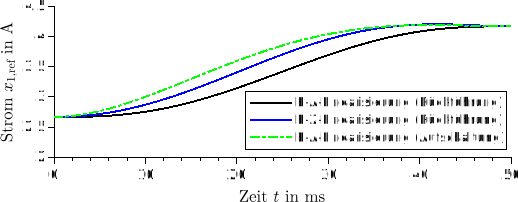
\includegraphics[width=0.8\textwidth]{Hochsetzsteller_Tracking_Strom}
\par\end{centering}
\caption{Ausgangsreferenzverläufe des Hochsetzstellers\label{fig:Hochsetzsteller-Tracking-Strom-FB-FF}}
\end{figure}


\section{Modellbasierte Regelung (IMC)\label{sec:Modellbasierte-Regelung-IMC}}

Die in diesem Buch behandelten Regelungsansätze sind alle modellbasiert
in dem Sinne, dass das Modell der Regelstrecke für den Reglerentwurf
benötigt wird.\footnote{Im Unterschied zu modellbasierten Verfahren gibt es auch Ansätze zur
\emph{modellfreien} Steuerung bzw. Regelung~\cite{fliess2009}. Bei
diesen Verfahren werden nur die Mess- oder Simulationsdaten genutzt.} Bei der \emph{modellbasierten Regelung}\index{modellbasierte Regelung}
(engl. \emph{internal model control}, kurz \emph{IMC}) im engeren
Sinne ist das Modell der Regelstrecke unmittelbar im Regler enthalten.
Der eigentliche Reglerentwurf ist auch bei komplizierten Modellen
vergleichsweise einfach und ähnelt der Entwurf einer Steuerung. Daher
ist dieser Ansatz u.\,a. in der chemischen Verfahrenstechnik sehr
beliebt. In Abschnitt~\ref{subsec:Modellbasierte-Regelung-linear}
wird zunächst der Reglerentwurf für lineare Regelstrecken vorgestellt~\cite{garcia1982}.
Die Verallgemeinerung auf nichtlineare Regelstrecken erfolgt in Abschnitt~\ref{subsec:Modellbasierte-Regelung-nichtlinear-minimalphasig}.

\subsection{Modellbasierte Regelung für lineare Systeme\label{subsec:Modellbasierte-Regelung-linear}}

Die Regelstrecke werde im Laplace-Bereich durch 
\[
Y(s)=G(s)\,U(s)+D(s)
\]
mit einer gebrochen rationalen, properen\index{Ubertragungsfunktion@{\"U}bertragungsfunktion!proper}\footnote{Eine rationale Übertragungsfunktion heißt \emph{proper}, wenn der
Grad des Zählerpolynoms nicht größer ist als der Grad des Nennerpolynoms.} Übertragungsfunktion~$G$, dem Eingang~$U$, dem Ausgang~$Y$
und der Störung~$D$ beschrieben. Abb.~\ref{fig:Struktur-IMC-linear}
zeigt die bei der modellbasierten Regelung verwendete Anordnung~\cite{lunze2007}.
Der Gesamtregeler besteht dabei aus einem sog. \emph{IMC-Regler} mit
der Übertragungsfunktion~$K$ und einem durch die Übertragungsfunktion~$\hat{G}$
beschriebenen Modell der Regelstrecke.
\begin{figure}
\begin{centering}
\resizebox{0.75\textwidth}{!}{\input{IMC-linear.pdftex_t}}
\par\end{centering}
\caption{Struktur einer modellbasierten Regelung\label{fig:Struktur-IMC-linear}}
\end{figure}

Bei der modellbasierten Regelung wird der Streckenausgang~$y$ mit
dem Modellausgang~$\hat{y}$ verglichen. Bei exakter Modellkenntnis
($G=\hat{G}$) reduziert sich im störungsfreien Fall ($d=0$) der
in Abb.~\ref{fig:Struktur-IMC-linear} gezeigte Regelkreis wegen
$y=\hat{y}$ auf eine reine Steuerung, wobei der IMC-Regler als Steuerungseinrichtung
bzw. Vorfilter fungiert (siehe Abb.~\ref{fig:Struktur-IMC-Steuerung}).
Für die Stabilität des Gesamtsystems ergibt sich sofort die Forderung,
dass sowohl die Regelstrecke als auch der Regler stabil sein müssen. 

\begin{figure}
\begin{centering}
\resizebox{0.65\textwidth}{!}{\input{IMC-linear-Steuerung.pdftex_t}}
\par\end{centering}
\caption{Vereinfachung einer modellbasierten Regelung zur Steuerung\label{fig:Struktur-IMC-Steuerung}}
\end{figure}

Bei der Steuerung in Abb.~\ref{fig:Struktur-IMC-Steuerung} würde
man mit der Wahl 
\begin{equation}
K(s)=G^{-1}(s)\label{eq:IMC-perfekter-Regler-linear}
\end{equation}
die Dynamik der Regelstrecke exakt kompensieren. Der Ausgang~$y$
würde (nach dem einmaligen Einschwingen durch verschiedene Anfangswerte
von Strecke und Steuerung) der Führungsgröße unmittelbar folgen. Man
spricht daher von einem \emph{perfekten} \emph{IMC-Regler}~\cite{garcia1982}.
Der perfekte Regler~(\ref{eq:IMC-perfekter-Regler-linear}) ist jedoch
aus folgenden Gründen meistens nicht einsetzbar:
\begin{enumerate}
\item \label{enu:IMC-Problem1}Ist der Zählergrad der Streckenübertragungsfunktion~$G$
echt kleiner als der Nennergrad, dann sind die Verhältnisse bei der
inversen Übertragungsfunktion~$G^{-1}$ umgekehrt, so dass der Zählergrad
größer als der Nennergrad ist. Eine derartige Reglerübertragungsfunktion~(\ref{eq:IMC-perfekter-Regler-linear})
wäre nicht mehr proper. 
\item \label{enu:IMC-Problem2}Bei der Inversion~(\ref{eq:IMC-perfekter-Regler-linear})
gehen die Nullstellen von~$G$ in die Polstellen von~$G^{-1}$ über.
Liegen Nullstellen von~$G$ in der rechten Halbebene, dann besitzt
das inverse Modell~$G^{-1}$ Polstellen in der rechten Halbebene
und ist daher instabil.
\end{enumerate}

Das erste Problem lässt sich umgehen, wenn man den IMC-Regler zusätzlich
mit einem Filter ausstattet. Sei $r>0$ die Differenz zwischen Zähler-
und Nennergrad von~$G$, d.\,h. das durch die Übertragungsfunktion~$G$
beschriebene Modell hat den relativen Grad~$r$ (vgl. Anmerkung~\ref{rem:rel-grad-Uebertragungsfunktion}).
Setzt man für das Filter die Übertragungsfunktion
\begin{equation}
F(s)=\frac{a_{0}}{a_{0}+a_{1}s+\cdots+a_{r-1}s^{r-1}+s^{r}}\label{eq:IMC-Filter-F}
\end{equation}
mit einem stabilen Nennerpolynom an, so ist der neue IMC-Regler
\begin{equation}
K(s)=F(s)\cdot G^{-1}(s)\label{eq:IMC-Regler-mit-Filter-linear}
\end{equation}
proper, d.\,h. der Zähler von~$K$ weist keinen Gradüberschuss mehr
auf. 

Eine stabile Übertragungsfunktion
\begin{equation}
G(s)=\frac{Z(s)}{N(s)}=\frac{\bar{b}_{0}+\bar{b}_{1}s+\bar{b}_{2}s^{2}+\cdots+\bar{b}_{n-r}s^{n-r}}{\bar{a}_{0}+\bar{a}_{1}s+\cdots+\bar{a}_{n-1}s^{n-1}+s^{n}}\label{eq:IMC-P}
\end{equation}
nennt man \emph{minimalphasig}\footnote{Die Verbindung zur Minimalphasigkeit in Sinne der Nulldynamik wird
in Anmerkung~\ref{rem:Nulldynamik-Nullstellen-Uebertragungsfunktion}
beschrieben.}\index{Ubertragungsfunktion@{\"U}bertragungsfunktion!minimalphasig}\index{minimalphasig},
wenn alle Nullstellen des Zählerpolynoms $Z(s)$ in der offenen linken
Halbebene liegen. Für eine minimalphasige Streckenübertragungsfunktion
ist der IMC-Regler~(\ref{eq:IMC-Regler-mit-Filter-linear}) auch
stabil. Andernfalls kann man die Übertragungsfunktion~$G$ in einen
minimalphasigen Anteil~$G_{\text{MP}}$ und einen Allpass~$G_{\text{A}}$
zerlegen~\cite{lunze2007}:
\begin{equation}
G(s)=G_{\text{MP}}(s)\cdot G_{\text{A}}(s).\label{eq:zerlegung-minimalphasig-allpass}
\end{equation}
Der IMC-Regler hat dann die Form
\begin{equation}
K(s)=F(s)\cdot G_{\text{MP}}^{-1}(s).\label{eq:IMC-Regler-mit-Filter-minimalphasig}
\end{equation}
Diesen Ansatz kann man als stabile Approximation der inversen Strecken\-dynamik~(\ref{eq:IMC-perfekter-Regler-linear})
auffassen.

\begin{remark}
\label{rem:Uebertragungsfunktion-minimalphasiger-Anteil}Bei einer
nicht minimal\-phasigen Übertragungsfunktion~$G$ erhält man den
minimal\-phasigen Anteil~$G_{\text{MP}}$ dadurch, dass man die
in der rechten Halbebene liegenden Nullstellen an der imaginären Achse
spiegelt. Da die Nullstellen entweder reell sind oder in konjugiert
komplexen Paaren auftreten, kann diese Spiegelung auch am Ursprung
erfolgen. Liegen \textit{alle} Nullstellen in der rechten Halbebene,
so heißt die Übertragungsfunktion \emph{maximal\-phasig}\index{Ubertragungsfunktion@{\"U}bertragungsfunktion!maximalphasig}\index{maximalphasig}~\cite{doyle96}.
In diesem Fall erhält man für die Übertragungsfunktion~(\ref{eq:IMC-P})
den minimal\-phasigen Anteil 
\begin{equation}
G_{\text{MP}}(s)=\frac{Z(-s)}{N(s)}=\frac{\bar{b}_{0}-\bar{b}_{1}s+\bar{b}_{2}s^{2}-\cdots+\bar{b}_{n-r}(-s)^{n-r}}{\bar{a}_{0}+\bar{a}_{1}s+\cdots+\bar{a}_{n-1}s^{n-1}+s^{n}},\label{eq:IMC-PMP}
\end{equation}
durch die Substitution $s\mapsto-s$ im Zählerpolynom.
\end{remark}

\begin{example}
\label{exa:IMC-linear}Die Übertragungsfunktion
\[
G(s)=\frac{3-s}{(s+1)(s+2)}
\]
der Regelstrecke ist selber stabil, ihre Inverse~$G^{-1}$ wegen
der o.\,g. Probleme~\ref{enu:IMC-Problem1} und~\ref{enu:IMC-Problem2}
dagegen nicht. Eine Zerlegung nach Gl.~(\ref{eq:zerlegung-minimalphasig-allpass})
liefert 
\[
G(s)=\underbrace{\frac{3+s}{(s+1)(s+2)}}_{{\displaystyle G_{\text{MP}}(s)}}\cdot\frac{3-s}{3+s}.
\]
Der Gradunterschied zwischen Nenner- und Zählerpolynom erfordert ein
Filter~(\ref{eq:IMC-Filter-F}) der Ordnung $r=1$. Damit erhält
man für den IMC-Regler~(\ref{eq:IMC-Regler-mit-Filter-minimalphasig})
die stabile Übertragungsfunktion
\[
K(s)=\frac{a_{0}}{s+a_{0}}\cdot\frac{(s+1)(s+2)}{3+s}
\]
mit einem Koeffizienten $a_{0}>0$.\footnote{Mit $a_{0}\in\{1,2\}$ kann man durch Pol-Nullstellen-Kürzung die
Ordnung des IMC-Reglers reduzieren. Für $a_{0}=1$ erhält man beispielsweise
$K(s)=\frac{s+2}{s+3}$.}
\end{example}

Die in Abb.~\ref{fig:Struktur-IMC-linear} gezeigte Anordnung einer
modellbasierten Regelung kann man in die Form eines Standardregelkreises
überführen (siehe Abb.~\ref{fig:IMC-linear-Standardregelkreis}).
Die gezeigte Regel\-kreis\-struktur lässt sich in ähnlicher Weise
auf nichtlineare Systeme übertragen.

\begin{figure}
\begin{centering}
\resizebox{0.8\textwidth}{!}{\input{IMC-linear-Standardregelkreis.pdftex_t}}
\par\end{centering}
\caption{Darstellung der modellbasierten Regelung als Standardregelkreis\label{fig:IMC-linear-Standardregelkreis}}
\end{figure}


\subsection{Modellbasierte Regelung für nichtlineare minimalphasige Systeme\label{subsec:Modellbasierte-Regelung-nichtlinear-minimalphasig}}

Das Konzept der modellbasierten Regelung lässt sich auf nichtlineare
Systeme verallgemeinern~\cite{economou1986,henson1991,schwarzmann2006,schwarzmann2007}.
Wir betrachten ein System~(\ref{eq:var-basissystem}) mit relativem
Grad~$r$. Das System sei minimalphasig und eingangs-zustands-stabil
(siehe Anhang~\ref{sec:Stabilitaet-erregter-Systeme}). 

Bei wohldefiniertem relativen Grad kann man das inverse Systemmodell
durch die Hirschorn-Inverse~(\ref{eq:hirschorn-inverse-SISO})\index{Hirschorn-Inverse}
realisieren (vgl. Anmerkung~\ref{rem:Hirschorn-Inverse}). Die Hirschorn-Inverse
benötigt neben der $r$-ten Zeitableitung des Ausgangs auch den Systemzustand.
Geht man zunächst von einer Systemdarstellung in der Byrnes-Isidori-Normalform~(\ref{eq:var-BI-NF})
aus, so ist auch der Zustand~$\xi$ des ersten Teilsystems nach Gl.~(\ref{eq:Zustand-xi-durch-y})
durch die Zeitableitungen des Ausgangs~$y$ darstellbar. Da Zeitableitungen
aus Mess\-signalen schwer zu ermitteln sind, schalten wir dem inversen
Systemmodell in Anlehnung an Gl.~(\ref{eq:IMC-Regler-mit-Filter-linear})
ein Filter vor. Die Übertragungsfunktion~(\ref{eq:IMC-Filter-F})
wird dabei als Zustandsraummodell 
\begin{equation}
\left.\begin{array}{lcl}
\dot{\hat{\xi}}_{1} & = & \hat{\xi}_{2}\\
 & \vdots\\
\dot{\hat{\xi}}_{r-1} & = & \hat{\xi}_{r}\\
\dot{\hat{\xi}}_{r} & = & -a_{0}\hat{\xi}_{1}-\cdots-a_{r-1}\hat{\xi}_{r}+a_{0}\tilde{w}\\
\hat{y} & = & \hat{\xi}_{1}
\end{array}\right\} \quad\begin{array}{lcl}
\dot{\hat{\xi}} & = & \left(A-bk^{T}\right)\hat{\xi}+a_{0}b\,\tilde{w}\\
\hat{y} & = & c^{T}\hat{\xi}
\end{array}\label{eq:IMC-Zustandsvariablenfilter}
\end{equation}
mit $k=(a_{0},\ldots,a_{r-1})^{T}$ implementiert, so dass sich der
Modellausgang~$\hat{y}$ und seine Zeitableitungen aus 
\[
\hat{y}=\hat{\xi}_{1},\;\dot{\hat{y}}=\hat{\xi}_{2},\;\ldots,\;\hat{y}^{(r-1)}=\hat{\xi}_{r},\;\hat{y}^{(r)}=-a_{0}\hat{\xi}_{1}-\cdots-a_{r-1}\hat{\xi}_{r}+a_{0}\tilde{w}
\]
ergeben. Man spricht hierbei von einem \emph{Zustandsvariablenfilter}\index{Zustandsvariablenfilter}~\cite{isermann2}.
Dabei wird aus dem Referenzsignal~$\tilde{w}$ ein geglätteter Zeitverlauf~$\hat{y}$
generiert, den man wie einen Referenzausgang aus Abschnitt~\ref{sec:Trajektorienfolgeregelung-Feedback}
behandeln kann. Den von dem Filter~(\ref{eq:IMC-Zustandsvariablenfilter})
bereitgestellten Zustand~$\hat{\xi}$ speist man in das zweite Teilsystem
der Byrnes-Isidori-Normalform
\[
\dot{\hat{\eta}}=q(\hat{\xi},\hat{\eta})
\]
ein und erhält damit einen Referenzverlauf~$\hat{\eta}$. Aus der
letzten Zeile des ersten Teilsystems erhält man den Eingang 
\begin{equation}
u=\frac{1}{\beta(\hat{\xi},\hat{\eta})}\left(\hat{y}^{(r)}-\alpha(\hat{\xi},\hat{\eta})\right).\label{eq:IMC-u}
\end{equation}
Mit der Rücktransformation $\hat{x}=\Phi^{-1}(\hat{\xi},\hat{\eta})$
kann man~(\ref{eq:IMC-u}) auch in Originalkoordinaten darstellen
und erhält dabei die Hirschorn-Inverse~(\ref{eq:hirschorn-inverse-SISO}).

Verwendet man anstelle der Byrnes-Isidori-Normalform~(\ref{eq:var-BI-NF})
die in der Regel leichter zu berechnende Eingangs-Ausgangs-Normalform~(\ref{eq:var-EA-NF}),
dann muss man erst den Eingang nach Gl.~(\ref{eq:IMC-u}) berechnen
und dann in das zweite Teilsystem einsetzen: 
\begin{equation}
\dot{\hat{\eta}}=q(\hat{\xi},\hat{\eta})+d(\hat{\xi},\hat{\eta})u.\label{eq:IMC-TS2-EA}
\end{equation}

Gleichungen~(\ref{eq:IMC-Zustandsvariablenfilter}), (\ref{eq:IMC-u})
und~(\ref{eq:IMC-TS2-EA}) bilden den IMC-Regler. Der Modell\-ausgang~$\hat{y}$
liegt dabei schon am Filter~(\ref{eq:IMC-Zustandsvariablenfilter})
an, so dass das Streckenmodell nicht noch separat zu implementieren
ist. Abb.~\ref{fig:Regelkreis-IMC-nichtlinear} zeigt den Regelkreis
für das nichtlineare System~(\ref{eq:var-basissystem}) in Verallgemeinerung
von Abb.~\ref{fig:IMC-linear-Standardregelkreis}. 

\begin{figure}
\begin{centering}
\resizebox{1\textwidth}{!}{\input{IMC-nichtlinear.pdftex_t}}
\par\end{centering}
\caption{Regelkreis mit nichtlinearem IMC-Regler für eine minimalphasige Regelstrecke\label{fig:Regelkreis-IMC-nichtlinear}}

\end{figure}

\begin{example}
\label{exa:hochsetzsteller-IMC}Wir betrachten wieder den \index{Hochsetzsteller}Hochsetzsteller~(\ref{eq:var-hochsetzsteller})
mit dem Strom als Ausgang entsprechend Gl.~(\ref{eq:hochsetzsteller-ausgang-strom-tracking}).
Das System hat den relativen Grad $r=1$ und liegt schon in der Eingangs-Ausgangs-Normalform~(\ref{eq:var-EA-NF})
mit $\xi_{1}=x_{1}$ und $\eta_{1}=x_{2}$ vor. In der Implementierung
bietet sich daher die Verwendung der ursprünglichen Bezeichnungen
für die Zustandsvariablen an. Das Zustandsvariablenfilter~(\ref{eq:IMC-Zustandsvariablenfilter})
wird als Filter erster Ordnung
\begin{equation}
\dot{\hat{x}}_{1}=a_{0}\left(\tilde{w}-\hat{x}_{1}\right),\quad\tilde{w}=w-\left(y-\hat{x}_{1}\right)\label{eq:hochsetzsteller-IMC-x1hat}
\end{equation}
mit einem Koeffizienten $a_{0}>0$ angesetzt. Das Umstellen der ersten
Systemgleichung von~(\ref{eq:var-hochsetzsteller}) liefert die Hirschorn-Inverse
\begin{equation}
u=\frac{\hat{x}_{2}-E+L\dot{\hat{x}}_{1}}{\hat{x}_{2}}\label{eq:hochsetzsteller-IMC-u}
\end{equation}
nach Gl.~(\ref{eq:IMC-u}). Das damit erzeugte Eingangssignal speist
man in die zweite Systemgleichung von~(\ref{eq:var-hochsetzsteller})
ein, um den Verlauf von~$x_{2}$ im Regler zu simulieren: 
\begin{equation}
\dot{\hat{x}}_{2}=(1-u)\frac{1}{C}\hat{x}_{1}-\frac{1}{RC}\hat{x}_{2}.\label{eq:hochsetzsteller-IMC-x2hat}
\end{equation}
Gleichzeitig ist~(\ref{eq:hochsetzsteller-IMC-u}) das Reglerausgangssignal,
welches in die Regelstrecke~(\ref{eq:var-hochsetzsteller}) eingespeist
wird.

Für die numerische Simulation wird wieder der Übergang von $20\,\text{V}$
auf $25\,\text{V}$ betrachtet. Dazu wird das Führungssignal 
\[
w(t)=\left\{ \begin{array}{rcl}
2,\bar{6}\,\text{A} & \text{für} & t<50\,\text{ms}\\
4,1\bar{6}\,\text{A} & \text{für} & t\geq50\,\text{ms}
\end{array}\right.
\]
vorgegeben. Für den Hochsetzsteller werden die von der Ruhelage abweichenden
Anfangswerte $x_{1}(0)=2\,\text{A}$ und $x_{2}(0)=15\,\text{V}$
vorgegeben, für den aus den Differentialgleichungen~(\ref{eq:hochsetzsteller-IMC-x1hat})
und~(\ref{eq:hochsetzsteller-IMC-x2hat}) bestehenden IMC-Regler
dagegen die Anfangswerte $\hat{x}_{1}(0)=2,\bar{6}\,\text{A}$ und
$\hat{x}_{2}(0)=20\,\text{\text{V}}$. Wie in Abschnitt~\ref{subsec:Hochsetzsteller-Num-Sim}
wird der normierte Filterparameter $a_{0}=300$ eingesetzt. Abb.~\ref{fig:Hochsetzsteller-IMC-Strom}
zeigt das Simulationsergebnis. Durch die unterschiedlichen Anfangswerte~$x(0)$
bzw.~$\hat{x}(0)$ treten zunächst Schwingungen auf, die bei dem
ab $t=50\,\text{ms}$ eingeleiteten Übergang der Ausgangsspannung
weitgehend abgeklungen sind.
\end{example}
\begin{figure}
\begin{centering}
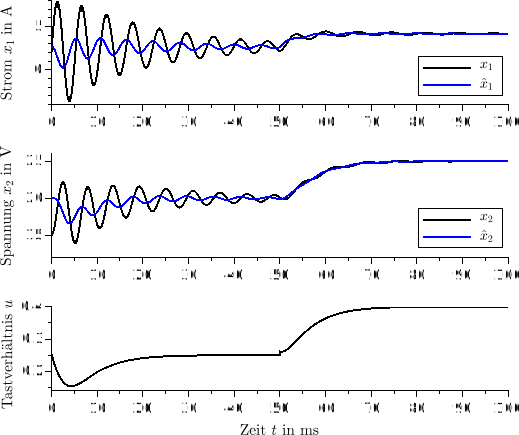
\includegraphics[width=0.8\textwidth]{Hochsetzsteller_IMC_Strom}
\par\end{centering}
\caption{Simulation des Hochsetzstellers mit dem IMC-Regler aus Beispiel~\ref{exa:hochsetzsteller-IMC}\label{fig:Hochsetzsteller-IMC-Strom}}
\end{figure}


\subsection{Modellbasierte Regelung für nichtlineare maximalphasige Systeme\label{subsec:Modellbasierte-Regelung-nichtlinear-maximalphasig}}

Die zur IMC-Regelung verwendete Aufspaltung einer nicht minimalphasigen
Übertragungsfunktion in einen minimalphasigen Anteil und einen Allpass
lässt sich prinzipiell auch auf nichtlineare Systeme übertragen, ist
in der Regel aber sehr kompliziert~\cite{ball2004}. In Anlehnung
an~\cite{doyle96} wird in diesem Abschnitt eine Methode zur IMC-Regelung
einer speziellen Klasse nicht minimalphasiger Systeme vorgestellt.

Wir betrachten ein System~(\ref{eq:var-basissystem}) mit einem wohldefinierten
relativen Grad $r<n$. Damit kann das Systm in die Byrnes-Isidori-Normalform~(\ref{eq:var-BI-NF})
transformiert werden. Das System ist minimalphasig\index{minimalphasig},
wenn die Ruhelage $\eta=0$ der Nulldynamik
\begin{equation}
\dot{\eta}=q(0,\eta)\label{eq:var-nulldynamik}
\end{equation}
asymptotisch stabil ist (vgl. Abschnitt~\ref{subsec:Reglerentwurf-zur-Stabilisierung-Ruhelage}).
Ist die Ruhelage zusätzlich hyperbolisch\index{Ruhelage!hyperbolische},
dann liegen alle $n-r$ Eigenwerte der aus der Taylor-Linearisierung
resultierenden Matrix 
\begin{equation}
A_{22}:=\left.\frac{\partial}{\partial\eta}q(0,\eta)\right|_{\eta=0}\label{eq:eq:var-nulldynamik-linearisierung}
\end{equation}
in der offenen linken Halbebene (vgl. Anmerkungen~\ref{rem:Nulldynamik-linear}
und~\ref{rem:Nulldynamik-Nullstellen-Uebertragungsfunktion}).

In Anlehnung an~\cite{doyle96} nennen wir ein System \emph{maximalphasig}\index{maximalphasig},
wenn die Ruhelage $\eta=0$ des zur Nulldynamik~(\ref{eq:var-nulldynamik})
assoziierten Systems 
\begin{equation}
\dot{\eta}=-q(0,\eta)\label{eq:nulldynamik-maximalphasig}
\end{equation}
asymptotisch stabil ist. Im Falle einer hyperbolischen Ruhelage liegen
dann alle Eigenwerte der zugehörigen Jacobimatrix
\[
\left.\frac{\partial}{\partial\eta}\left(-q(0,\eta)\right)\right|_{\eta=0}=-\left.\frac{\partial}{\partial\eta}q(0,\eta)\right|_{\eta=0}=-A_{22}
\]
in der offenen linken Halbebene. Das bedeutet, dass alle Eigenwerte
der Jacobi\-matrix~(\ref{eq:eq:var-nulldynamik-linearisierung})
der ursprünglichen Nulldynamik~(\ref{eq:var-nulldynamik}) in der
offenen rechten Halbebene liegen.

Zusätzlich zur Byrnes-Isidori-Normalform betrachten wir das System~(\ref{eq:var-basissystem})
in der verallgemeinerten Regelungsnormalform\index{verallgemeinerte Regelungsnormalform}\index{Normalform!verallgemeinerte Regelungs-}
\begin{equation}
\begin{array}{lcl}
\dot{z}_{1} & = & z_{2}\\
 & \vdots\\
\dot{z}_{n-1} & = & z_{n}\\
\dot{z}_{n} & = & \underbrace{\alpha\left(z,u,\dot{u},\ddot{u},\ldots,u^{(n-r-1)}\right)+\beta\left(z,u,\dot{u},\ddot{u},\ldots,u^{(n-r-1)})\right)u^{(n-r)}}_{{\displaystyle \delta\left(u,\dot{u},\ldots,u^{(n-r)}\right)}}\\
y & = & z_{1},
\end{array}\label{eq:var-verallgemeinerte-Regelungsnormalform-maxmalphasig}
\end{equation}
vgl. Abschnitt~\ref{subsec:Verallgemeinerte-Regelungsnormalform}.
Da das Ausgangssystem~(\ref{eq:var-basissystem}) affin ist, ist
die in der letzten Differentialgleichung von~(\ref{eq:var-verallgemeinerte-Regelungsnormalform-maxmalphasig})
auftretende Nichtlinearität~$\delta$ affin bezüglich der höchsten
Zeitableitung des Eingangs. Die Transformation $z=\Phi(x,u,\dot{u},\ldots,u^{(n-r-1)})$
ergibt sich aus Zeitableitungen $z_{1}=y,\,z_{2}=\dot{y},\,z_{3}=\ddot{y},\ldots,\,z_{n}=y^{(n-1)}$.

Die Linearierung von System~(\ref{eq:var-verallgemeinerte-Regelungsnormalform-maxmalphasig})
führt auf eine Übertragungsfunktion~$G(s)$ der Form~(\ref{eq:IMC-P}).
Die Koeffizienten $\bar{b}_{0},\ldots,\bar{b}_{n-r}$ des Zählerpolynoms
$Z(s)$ ergeben sich dabei aus den partiellen Ableitungen von~$\delta$
nach dem Eingang und seien Zeitableitungen, d.\,h. 
\begin{equation}
\bar{b}_{0}=\frac{\partial\delta}{\partial u},\;\bar{b}_{1}=\frac{\partial\delta}{\partial\dot{u}},\;\ldots,\bar{b}_{n-r}=\frac{\partial\delta}{\partial u^{(n-r)}}\label{eq:IMC-koeff-nennerpolynom}
\end{equation}
für $z=0,u=0,\ldots,u^{(n-r)}=0$. Bei einem maximalphasigen System
mit hyperbolischer Ruhelage liegen alle Nullstellen des Zählerpoylnoms
$Z(s)$ in der rechten Halbebene. Der Übergang von $Z(s)$ zu $Z(-s)$
liefert den minimalphasigen Anteil~(\ref{eq:IMC-PMP}) der Übertragungsfunktion~(\ref{eq:IMC-P}),
vgl. Anmerkung~\ref{rem:Uebertragungsfunktion-minimalphasiger-Anteil}.
Diesen Ansatz übertragen wir jetzt auf das nichtlineare System~(\ref{eq:var-verallgemeinerte-Regelungsnormalform-maxmalphasig}).
Die im Zählerpolynom der Übertragungsfunktion durchgeführte Ersetzung
$s\mapsto-s$ entspricht wegen~(\ref{eq:IMC-koeff-nennerpolynom})
in der Nichtlinearität~$\delta$ der Substitution $\tfrac{\d}{\d t}\mapsto-\tfrac{\d}{\d t}$.
Im Falle eines maximalphasigen Systems~(\ref{eq:var-verallgemeinerte-Regelungsnormalform-maxmalphasig})
erhält man dadurch den zugehörigen minimalphasigen Anteil
\begin{equation}
\begin{array}{lcl}
\dot{z}_{1} & = & z_{2}\\
 & \vdots\\
\dot{z}_{n-1} & = & z_{n}\\
\dot{z}_{n} & = & \alpha\left(z,u,-\dot{u},\ddot{u},\ldots,(-1)^{n-r-1}u^{(n-r-1)}\right)\\
 &  & +(-1)^{n-r}\beta\left(z,u,-\dot{u},\ddot{u},\ldots,(-1)^{n-r-1}u^{(n-r-1)}\right)u^{(n-r)}\\
y & = & z_{1}.
\end{array}\label{eq:var-verallgemeinerte-Regelungsnormalform-minimalphasig}
\end{equation}
Die Lineariserung des resultierenden minimalphasigen Systems~(\ref{eq:var-verallgemeinerte-Regelungsnormalform-minimalphasig})
liefert unmittelbar die Übertragungsfunktion $G_{\text{MP}}(s)$ analog
zu Gl.~(\ref{eq:IMC-PMP}):

\[
\begin{CD}
\text{System}~\eqref{eq:var-verallgemeinerte-Regelungsnormalform-maxmalphasig} @>{\displaystyle\text{Zerlegung}}>>\text{System}~\eqref{eq:var-verallgemeinerte-Regelungsnormalform-minimalphasig}\\
@V{\displaystyle\text{Linearisierung}}VV @VV{\displaystyle\text{Linearisierung}}V\\
G(s) @>>{\displaystyle\text{Zerlegung}}> G_\text{MP}(s)
\end{CD}
\]

Zur Verallgemeinerung des linearen IMC-Reglers~(\ref{eq:IMC-Regler-mit-Filter-minimalphasig})
auf den nichtlinearen Fall lösen wir die letzte Differentialgleichung
von~(\ref{eq:var-verallgemeinerte-Regelungsnormalform-minimalphasig})
unter Beachtung von $\dot{z}_{n}=y^{(n)}$ nach der höchsten Zeitableitung
des Eingangs auf:
\begin{equation}
u^{(n-r)}=\left(-1\right)^{n-r}\,\frac{y^{(n)}-\alpha\left(z,u,-\dot{u},\ddot{u},\ldots,(-1)^{n-r-1}u^{(n-r-1)}\right)}{\beta\left(z,u,-\dot{u},\ddot{u},\ldots,(-1)^{n-r-1}u^{(n-r-1)}\right)u^{(n-r)}}.\label{eq:IMC-max-inv}
\end{equation}
Der Zustand~$z$ und die Zeitableitung~$y^{(n)}$ werden durch ein
Zustandsvariablenfilter der Struktur~(\ref{eq:IMC-Zustandsvariablenfilter}),
aber der Ordnung~$n$, mit dem Zustand~$\hat{z}$ geschätzt:
\begin{equation}
\begin{array}{lcl}
\dot{\hat{z}} & = & \left(A-bk^{T}\right)\hat{z}+a_{0}b\,\tilde{w}\\
\hat{y} & = & c^{T}\hat{z}.
\end{array}\label{eq:Filter-maximalphasig}
\end{equation}
Die so erhaltenen Schätzgrößen setzt man in Gl.~(\ref{eq:IMC-max-inv})
ein. Die Ableitung~$u^{(n-r)}$ führt man einer Integratorkette der
Länge $n-r$ zu, womit man die in Gl.~(\ref{eq:IMC-max-inv}) benötigten
Ableitungen $u^{(n-r-1)},\ldots,\dot{u}$ und auch den Eingang~$u$
als Stellgröße für die Regelstrecke~(\ref{eq:var-basissystem}) erhält.
Das dadurch entstehende Regelungsschema ist in Abb.~\ref{fig:Regelkreis-IMC-maximalphasig}
dargestellt.

\begin{figure}
\begin{centering}
\resizebox{1\textwidth}{!}{\input{IMC-maximalphasig.pdftex_t}}
\par\end{centering}
\caption{Regelkreis mit IMC-Regler eine für maximalphasige Regelstrecke\label{fig:Regelkreis-IMC-maximalphasig}}
\end{figure}

\begin{example}
\label{exa:Hochsetzsteller-IMC-Spannung}\index{Hochsetzsteller}Betrachtet
wird wieder der Hochsetzsteller. Wir verwenden die Kondensatorspannung~$x_{2}$
gleichzeitig als Ausgang wie auch als erste Koordinate des transformierten
Systems:
\begin{equation}
z_{1}=y=h(x)=x_{2}.\label{eq:IMC-hochsetzsteller-ausgang-spannung}
\end{equation}
Die zweite Koordinate ist die Zeitableitung des Ausgangs
\begin{equation}
z_{2}=\dot{y}=L_{f}h(x)+L_{g}h(x)u=(1-u)\frac{1}{C}x_{1}-\frac{1}{RC}x_{2},\label{eq:IMC-hochsetzsteller-ausgangsableitung}
\end{equation}
die vom Eingang~$u$ abhängt, so dass das System den relativen Grad
$r=1$ besitzt. Gln.~(\ref{eq:IMC-hochsetzsteller-ausgang-spannung})
und~(\ref{eq:IMC-hochsetzsteller-ausgangsableitung}) bilden eine
vom Eingang abhängige Koordinatentransformation $z=\Phi(x,u)$ mit
der Rücktransformation
\[
x_{1}=-\frac{z_{1}+RCz_{2}}{(u-1)R},\quad x_{2}=z_{1}.
\]
Aus der zweiten Zeitableitung des Ausgangs
\begin{eqnarray*}
\ddot{y} & = & L_{f}^{2}h(x)+\left(L_{g}L_{f}h(x)+L_{f}L_{g}h(x)\right)u+L_{g}^{2}h(x)u^{2}+L_{g}h(x)\dot{u}\\
 & = & -\frac{-Lx_{2}-\left(u-1\right)x_{1}LR+\left(L\dot{u}x_{1}+uE-E+u^{2}x_{2}-2ux_{2}+x_{2}\right)CR^{2}}{C^{2}LR^{2}}\\
 & = & \underbrace{-\frac{Lz_{2}+\left(u-1\right)\left(E+\left(u-1\right)\,z_{1}\right)R}{CLR}}_{{\displaystyle \alpha(z,u)}}+\underbrace{\frac{z_{1}+RCz_{2}}{(u-1)RC}}_{{\displaystyle \beta(z,u)}}\dot{u}
\end{eqnarray*}
erhält man die letzte Zeile der verallgemeinerten Regelungsnormalform:
\begin{equation}
\begin{array}{lcl}
\dot{z}_{1} & = & z_{2}\\
\dot{z}_{2} & = & \alpha(z,u)+\beta(z,u)\,\dot{u}\\
y & = & z_{1}
\end{array}\label{eq:hochsetzsteller-verallg-RNF1}
\end{equation}
Durch Zeitumkehr in der Eingangsdynamik, d.\,h. $\dot{u}\mapsto-\dot{u}$,
geht das nicht\-minimal\-phasige System~(\ref{eq:hochsetzsteller-verallg-RNF1})
in die minimalphasige Approximation
\begin{equation}
\begin{array}{lcl}
\dot{z}_{1} & = & z_{2}\\
\dot{z}_{2} & = & \alpha(z,u)-\beta(z,u)\,\dot{u}\\
y & = & z_{1}
\end{array}\label{eq:hochsetzsteller-verallg-RNF2}
\end{equation}
über. Stellt man die letzte Differentialgleichung in~(\ref{eq:hochsetzsteller-verallg-RNF2})
nach~$\dot{u}$ um, so erhält man 
\begin{equation}
\dot{u}=-\frac{\left(u-1\right)\left(z_{2}L+\left(\dot{z}_{2}CL+uE-E+u^{2}z_{1}-2uz_{1}+z_{1}\right)R\right)}{L\left(z_{2}CR+z_{1}\right)}.\label{eq:hochsetzsteller-maximalphasig-du}
\end{equation}
Die Größen $z_{1},z_{2},\dot{z}_{2}$ lassen sich durch $y,\dot{y},\ddot{y}$
repräsentieren. Im IMC-Regler verwendet man dafür die vom Zustandsvariablenfilter
\begin{equation}
\begin{array}{lcl}
\dot{\hat{z}}_{1} & = & \hat{z}_{2}\\
\dot{\hat{z}}_{2} & = & -a_{0}\hat{z}_{1}-a_{1}\hat{z}_{2}+a_{0}\tilde{w}\\
\hat{y} & = & \hat{z}_{1}
\end{array}\label{eq:hochsetzsteller-maxphas-zustandsvarfilter}
\end{equation}
mit $a_{0},a_{1}>0$ generierten Schätzsignale $\hat{y},\dot{\hat{y}},\ddot{\hat{y}}$.
Die Integration von~$\dot{u}$ aus Gl.~(\ref{eq:hochsetzsteller-maximalphasig-du})
liefert das Streckeneingangssignal~$u$. Mit~(\ref{eq:hochsetzsteller-maximalphasig-du})
und~(\ref{eq:hochsetzsteller-maxphas-zustandsvarfilter}) erhält
man insgesamt einen dynamischen Regler dritter Ordnung.

Für die numerische Simulation wird der Übergang von $20\,\text{V}$
auf $25\,\text{V}$ direkt durch das Führungssignal 
\[
w(t)=\left\{ \begin{array}{rcl}
20\,\text{V} & \text{für} & t<50\,\text{ms}\\
25\,\text{V} & \text{für} & t\geq50\,\text{ms}
\end{array}\right.
\]
vorgegeben. Wie in Beispiel~\ref{exa:hochsetzsteller-IMC} finden
für den Hochsetzsteller die Anfangswerte $x_{1}(0)=2\,\text{A}$ und
$x_{1}(0)=20\,\text{V}$ Verwendung. Die Anfangswerte des Zustandsvariablenfilters~(\ref{eq:hochsetzsteller-maxphas-zustandsvarfilter})
lauten $\hat{z}_{1}(0)=20$ und $\hat{z}_{2}(0)=0$. Für die Differentialgleichung~(\ref{eq:hochsetzsteller-maximalphasig-du})
des Eingangs gilt $u(0)=0,25$. Zusätzlich kommen die Filterkoeffizienten
$a_{0}=90000$ und $a_{1}=600$ aus Abschnitt~\ref{subsec:Hochsetzsteller-Num-Sim}
zum Einsatz. Abb.~\ref{fig:Hochsetzsteller-IMC-Spannung} zeigt die
simulierten Signalverläufe. Zunächst ist der Einschwingvorgang des
Hochsetzstellers festzustellen. Der Übergang der Ausgangsspannung
erfolgt wie gewünscht.
\end{example}
\begin{figure}
\begin{centering}
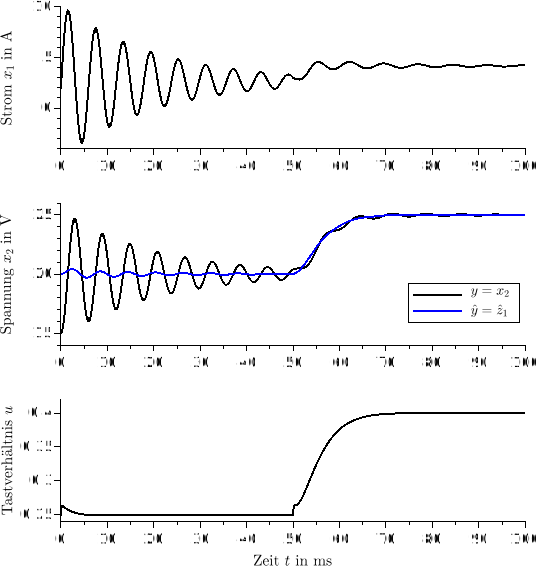
\includegraphics[width=0.8\textwidth]{Hochsetzsteller_IMC_Spannung}
\par\end{centering}
\caption{Simulation des Hochsetzstellers mit dem IMC-Regler aus Beispiel~\ref{exa:Hochsetzsteller-IMC-Spannung}\ref{exa:hochsetzsteller-IMC}\label{fig:Hochsetzsteller-IMC-Spannung}}
\end{figure}


\section{Approximative Linearisierung durch Modifikation\label{sec:Approximative-Linearisierung-Modifikation}}

Bei den bisherigen Betrachtung wurde für das System~(\ref{eq:var-basissystem})
immer ein wohldefinierter relativer Grad vorausgesetzt. Andernfalls
ist die in Kapitel~\ref{chap:regler-grundlagen} beschriebene exakte
Linearisierung nicht (direkt) anwendbar. Mit dem in~\cite{hauser92}
vorgestellten Zugang wird bei nicht wohldefiniertem relativen Grad
eine approximative Linearisierung erzielt\index{Linearisierung!approximative}.

Der relative Grad von System~(\ref{eq:var-basissystem}) ist im Punkt
$p\in\mathcal{M}$ \textit{nicht} wohldefiniert, wenn die erste nicht
verschwindende Lie-Ableitung im Punkt~$p$ Null ist, d.\,h. 
\[
L_{g}L_{f}^{r-1}h(x)\not\equiv0,\quad\text{aber}\quad L_{g}L_{f}^{r-1}h(p)=0.
\]
Das bedeutet, dass beim ersten Auftreten des Eingangs in den Zeitableitungen
des Ausgangs 
\[
\begin{array}{lcl}
y & = & h(x)\\
 & \vdots\\
y^{(r-1)} & = & L_{f}^{r-1}h(x)\\
y^{(r)} & = & L_{f}^{r}h(x)+L_{g}L_{f}^{r-1}h(x)\,u
\end{array}
\]
der Faktor $L_{g}L_{f}^{r-1}h(x)$ vor dem Eingang~$u$ im Punkt~$p$
verschwindet. Aus Stetigkeitsgründen ist dann $L_{g}L_{f}^{r-1}h(x)$
für alle~$x$ aus einer (hinreichend kleinen) Umgebung von~$p$
auch betragsmäßig klein. Der in~\cite{hauser92} vorgestellte Ansatz
beruht darauf, dass man den Term $L_{g}L_{f}^{r-1}h(x)u$ vernachlässigt
und weiter differenziert. Diese Ableitungsbildung unter Vernachlässigung
des angegebenen Terms lässt sich über Lie-Ableitungen entlang des
Vektorfelds~$f$ darstellen. Unter dem sich dabei ergebenden Diffeomorphismus
$\xi=\Phi(x)$ mit $\xi_{1}=h(x),\,\xi_{2}=L_{f}h(x),\ldots,\xi_{n}=L_{f}^{n-1}h(x)$
erhält man das transformierte System
\begin{equation}
\begin{array}{lcl}
\dot{\xi}_{1} & = & \xi_{2}\\
 & \vdots\\
\dot{\xi}_{r-1} & = & \xi_{r}\\
\dot{\xi}_{r} & = & \xi_{r+1}+\beta_{r}(\xi)\,u\\
 & \vdots\\
\dot{\xi}_{n-1} & = & \xi_{n}+\beta_{n-1}(\xi)\,u\\
\dot{\xi}_{n} & = & \alpha_{n}(\xi)+\beta_{n}(\xi)\,u
\end{array}\label{eq:var-approx-ARNF}
\end{equation}
mit 
\[
\alpha_{n}(\xi)=L_{f}^{n}h(\Phi^{-1}(\xi)),\quad\beta_{i}(\xi)=L_{g}L_{f}^{i-1}h(\Phi^{-1}(\xi)),\quad i=r,\ldots,n.
\]

Für die approximative Linearisierung\index{Linearisierung!approximative}
nehmen wir an, dass die Terme $\beta_{r},\ldots\beta_{n-1}$ im betreffenden
Arbeitsbereich (betragsmäßig) kleine Werte annehmen, der Term~$\beta_{n}$
sich aber erheblich von der Null unterscheidet. Die Linearisierung
durch Rückführung führt man in der letzten Zeile von System~(\ref{eq:var-approx-ARNF})
mit dem fiktiven Eingang~$v$ durch:
\begin{equation}
v\stackrel{!}{=}\alpha_{n}(\xi)+\beta_{n}(\xi)\,u\quad\Longleftrightarrow\quad u=\frac{1}{\beta_{n}(\xi)}\left(v-\alpha_{n}(\xi)\right).\label{eq:var-approximativ-linearisierende-rueckfuehrung}
\end{equation}
Zur Stabilisierung kombiniert man die (approximativ) linearisierende
Rückführung~(\ref{eq:var-approximativ-linearisierende-rueckfuehrung})
mit der Rückführung $v=-k^{T}\xi$. Die Verstärkung $k^{T}=(a_{0},\ldots,a_{n})$
enthält die Koeffizienten eines vorgegebenen charakteristischen Polynoms
\begin{equation}
\det\left(sI-\left(A-bk^{T}\right)\right)=a_{0}+a_{1}s+\cdots+a_{n-1}s^{n-1}+s^{n}.\label{eq:var-al-char-poly}
\end{equation}
Somit erhält man für die Originalkoordinaten in Anlehnung an Abschnitt~\ref{sec:E-A-Linearisierung-affin}
das Regelgesetz
\begin{equation}
u=-\frac{1}{L_{g}L_{f}^{n-1}h(x)}\sum_{i=0}^{n}a_{i}L_{f}^{i}h(x)\quad\text{mit}\quad a_{n}:=1.\label{eq:var-approx-rueckfuehrung-x}
\end{equation}
In ähnlicher Weise lassen sich auch die in den Abschnitten~\ref{sec:Trajektorienfolgeregelung-Feedback}
und~\ref{sec:Trajektorienfolgeregelung-Feedforward} beschriebenen
Rückführungen für Trajektorienfolgeregelungen nutzen. Die Stabilisierung
des rückgeführten Systems kann man mit Überlegungen des High-Gain-Entwurfs
begründen (vgl. Kapitel~\ref{chap:High-Gain-Beobachter}). 

\medskip{}

Die approximative Linearisierung wird in~\cite{hauser92,sastry1999}
am Beispiel eines Balls auf einem Balken (engl. ball \& beam example)
untersucht. Dieses Beispiel wurde in etlichen weiteren Veröffentlichungen
aufgegriffen~\cite{leith2001,zhang2006feedback}. In~\cite{zimmer1995,sastry1998helicopter}
wird die approximtive Linearisierung eines Hubschraubermodells behandelt.
Das folgende Beispiel ist an~\cite{aguilar2002approximate} angelehnt:
\begin{example}
\label{exa:wagen-pendel-approximativ}Wir betrachten das partiell
linearisierte Modell des Wagen-Pendel-Systems aus Abschnitt~\ref{subsec:Wagen-mit-Pendel}
und Beispiel~\ref{exa:Wagen-Pendel-partielle-Linearisierung} unter
Vernachlässigung der Reibung:
\begin{equation}
\begin{array}{lcl}
\dot{x}_{1} & = & x_{2}\\
\dot{x}_{2} & = & v\\
\dot{x}_{3} & = & x_{4}\\
\dot{x}_{4} & = & -\frac{g}{l}\sin x_{3}-\frac{1}{l}v\cos x_{3}\\
y & = & x_{1}.
\end{array}\label{eq:var-approx-wagen-pendel-linearisiert}
\end{equation}
In Beispiel~\ref{exa:Wagen-Pendel-max-rel-grad} wurde für dieses
System der (fiktive) Ausgang
\begin{equation}
h(x)=x_{1}+\frac{l}{2}\ln\left(\frac{1+\sin x_{3}}{1-\sin x_{3}}\right)\label{eq:var-approx-wagen-ausgang-r-3}
\end{equation}
ermittelt, mit dem das System wegen $L_{g}h(x)=L_{g}L_{f}h(x)=0$
und $L_{g}L_{f}^{2}h(x)=-2x_{4}\tan x_{3}$ für $x_{3}\neq k\pi$,
$k\in\Z$ und $x_{4}\neq0$ den (maximalen) relativen Grad $r=3$
besitzt. Im Punkt $x=0$ ist der relative Grad damit nicht definiert.
Für die Approximation gehen wir von $x_{3}\approx0$ (kleine Auslenkung
des Pendels) und $x_{4}\approx0$ (kleine Winkelgeschindigkeit) aus
und bestimmen die gemischte Lie-Ableitung der nächsthöheren Ordnung:
\begin{equation}
L_{g}L_{f}^{3}h(x)=\frac{\left(3l\cos\left(2x_{3}\right)-9l\right)x_{4}^{2}+\left(\cos\left(3x_{3}\right)-3\cos x_{3}\right)g}{l\left(\cos\left(2x_{3}\right)+1\right)}.\label{eq:var-approx-wagen-gemischte-Lie-Ableitung}
\end{equation}
Mit $L_{g}L_{f}^{3}h(0)=-g/l$ ist dieser Term im Arbeitspunkt $x=0$
nicht vernachlässigbar. Für die Rückführung~(\ref{eq:var-approx-rueckfuehrung-x})
benötigt man neben~(\ref{eq:var-approx-wagen-gemischte-Lie-Ableitung})
und dem Ausgang~(\ref{eq:var-approx-wagen-ausgang-r-3}) noch die
Lie-Ableitungen
\[
\begin{array}{lcl}
L_{f}h(x) & = & x_{2}+\frac{lx_{4}}{\cos x_{3}}\\
L_{f}^{2}h(x) & = & \tan x_{3}\left(g+\frac{lx_{4}^{2}}{\cos x_{3}}\right)\\
L_{f}^{3}h(x) & = & 2gx_{4}\,\frac{1-\cos(2x_{3})}{1+\cos(2x_{3})}+lx_{4}^{3}\,\frac{1-\sin^{4}x_{3}}{\cos^{5}x_{3}}\\
L_{f}^{4}h(x) & = & 2lx_{4}^{4}\frac{\sin x_{3}}{\cos^{2}x_{3}}\left(\frac{6}{\cos^{2}x_{3}}-1\right)+3gx_{4}^{2}\sin x_{3}\left(\frac{4}{\cos^{2}x_{3}}-1\right)\\
 &  & +\,\frac{g^{2}}{l}\sin x_{3}\left(\frac{3}{\cos^{2}x_{3}}-2\right).
\end{array}
\]

Zur numerischen Simulation verwenden wir mit Ausnahme von $d_{1}=0$
und $d_{2}=0$ (Vernachlässigung der Reibung) die Parameter und Anfangswerte
aus Beispiel~\ref{exa:Wagen-Pendel-Stabilisierung-Simulation}. Die
Eigenwerte werden durch $s_{1,2}=-2$ und $s_{3,4}=-3$ vorgegeben.
Das Simulationsergebnis ist Abb.~\ref{fig:Simulation-Wagen-Pendel-Approx-Lin}
zu entnehmen. Im Unterschied zur Regelung mittels Eingangs-Ausgangs-Linearisierung
in Beispiel~\ref{exa:Wagen-Pendel-Stabilisierung-Simulation} wird
jetzt die Dynamik für alle Zustände eingeprägt. Im Vergleich zu Abb.~\ref{fig:Simulation-Wagen-Pendel-System}
erfolgt hier ein schnelleres Einschwingen.
\end{example}
\begin{figure}
\begin{centering}
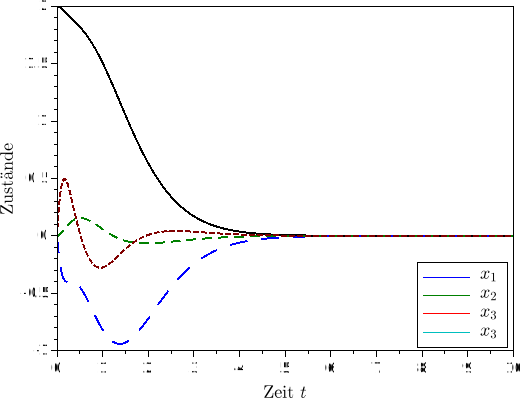
\includegraphics[width=0.85\textwidth]{Wagen_Pendel_Approx}
\par\end{centering}
\caption{Simulationsergebnis des geregelten Wagen-Pendel-Systems\label{fig:Simulation-Wagen-Pendel-Approx-Lin}}
\end{figure}

\begin{remark}
Den Reglerentwurf führt man nach Gl.~(\ref{eq:var-approx-rueckfuehrung-x})
so durch, als ob die Terme $\beta_{r},\ldots,\beta_{n-1}$ in Gl.~(\ref{eq:var-approx-ARNF})
identisch Null wären. Diese Annahme kann man auch als Modifikation
des Systems interpretieren, wodurch das resultierende System eingangs-zustands-linearisierbar
wird. Das Nullsetzen von $\beta_{r},\ldots,\beta_{n-1}$ in Gl.~(\ref{eq:var-approx-ARNF})
führt in Originalkoordinaten auf das modifizierte Vektorfeld 
\[
\tilde{g}(x)=\left[\Phi^{\prime}(x)\right]^{-1}\cdot\left.\beta_{n}(z)\frac{\partial}{\partial z_{n}}\right|_{z=\Phi(x)}=L_{g}L_{f}^{n-1}h(x)\cdot\left[\Phi^{\prime}(x)\right]^{-1}\cdot e_{n}.
\]
In ähnlicher Weise kann man auch durch Modifikation des Vektorfeldes~$f$
ein eingangs-zustands-linearisierbares System erzeugen~\cite{hauser92}.
\end{remark}

\section{Approximative Linearisierung durch Reihenentwicklung\label{sec:Approximative-Linearisierung-Reihenentwicklung}}

Um die einschränkenden Existenzbedingungen bzw. die schwierige Berechnung
für eine exakte Eingangs-Zustands-Linearisierung zu umgehen, wurden
in der Fachliteratur zahlreiche Approximationsansätze\index{Linearisierung!approximative}
vorgeschlagen~\cite{reboulet84,baumann86,guardabassi2001}. Etliche
Veröffentlichungen basieren auf einer Transformation des betreffenden
Systems in die Poincaré-Normalform\index{Normalform!Poincaré-}~\cite{krener84,krener90,krener91poincare,devanathan2001,devanathan2004}.
Dabei setzt man sowohl für das System als auch für die Transformation~$\Phi$
eine mehrvariable Taylor\-reihe an und versucht, die von den Nichtlinearitäten
herrührenden Terme höherer Ordnung schrittweise zu eliminieren. Da
die Anzahl der Terme einer mehrvariablen Taylorentwicklung exponentiell
mit der Entwicklungsordnung wächst, ist dieser Ansatz nur bedingt
praktikabel. 

Der in diesem Abschnitt vorgestellte Zugang nach~\cite{roebenack2012pamm,roebenack2013ecc,franke2015buch}
vermeidet die Reihenentwicklung der Koordinatentransformation und
kann in gewisser Weise als das Gegenstück zum erweiterten Luenberger-Beobachter
aufgefasst werden (vgl. Abschnitt~\ref{subsec:Luenberger}).

\subsection{Vorüberlegungen und exakte Linearisierung\label{subsec:Approx-exakt}}

Man betrachte eine eingangsaffine Regelstrecke 
\begin{equation}
\dot{x}=f(x)+g(x)\,u\label{eq:var-basissystem-ohne-ausgang}
\end{equation}
mit hinreichend glatten Vektorfeldern $f,g:\mathcal{M}\to\R^{n}$
auf einer offenen Menge $\mathcal{M}\subseteq\R^{n}$. Das System
ist in einem Punkt $p\in\mathcal{M}$ exakt eingangs-zustands-linearisierbar,
wenn es eine Ausgangsabbildung $h:\mathcal{M}\to\R$ gibt, für die
das System den relativen Grad~$n$ besitzt, also
\begin{equation}
L_{g}h(x)=0,\;L_{g}L_{f}h(x)=0,\;\ldots,\;L_{g}L_{f}^{n-2}h(x)=0,\;L_{g}L_{f}^{n-1}h(p)\neq0\label{eq:var-al-rel-grad-n-allgemein}
\end{equation}
für alle~$x$ aus einer Umgebung von~$p$ gilt (vgl. Abschnitt~\ref{sec:Exakte-Eingangs-Zustands-Linearisierung}).
Wir gehen im Folgenden von der etwas strengeren Bedingung
\begin{equation}
L_{g}h(x)=0,\;L_{g}L_{f}h(x)=0,\;\ldots,\;L_{g}L_{f}^{n-2}h(x)=0,\;L_{g}L_{f}^{n-1}h(x)=1\label{eq:var-al-rel-grad-n-speziell}
\end{equation}
für alle~$x$ aus einer Umgebung von~$p$ aus.\footnote{Gilt~(\ref{eq:var-al-rel-grad-n-allgemein}), dann kann die Bedingung~(\ref{eq:var-al-rel-grad-n-speziell})
immer durch eine zustandsäbhängige Eingangstransformation $u\mapsto\tfrac{1}{L_{g}L_{f}^{n-1}h(x)}u$
erzwungen werden (vgl. Abschnitt~\ref{subsec:EZ-Linearisierung-Formen}).} Die Ausgangsabbildung~$h$ ist die Lösung der (partiellen) Differentialgleichung
\begin{equation}
\d h(x)=\omega(x),\label{eq:var-al-dh-omega}
\end{equation}
wobei sich das Kovektorfeld~$\omega$ aus der Steuerbarkeitsmatrix\index{Steuerbarkeitsmatrix}\index{Matrix!Steuerbarkeits-}
\begin{equation}
Q_{S}(x)=\left(g(x),\ad_{-f}g(x),\ldots,\ad_{-f}^{n-1}g(x)\right)\label{eq:var-al-steuerbarkeitsmatrix}
\end{equation}
entsprechend
\begin{equation}
\omega(x)=e_{n}^{T}Q_{S}^{-1}(x)\label{eq:var-al-startkovektor}
\end{equation}
mit dem $n$-ten Einheitsvektor~$e_{n}$ ergibt. Kennt man die Abbildung~$h$,
dann lässt sich das System mit dem Diffeomorphismus 
\begin{equation}
\xi=\Phi(x)=\left(\begin{array}{c}
h(x)\\
L_{f}h(x)\\
\vdots\\
L_{f}^{n-1}h(x)
\end{array}\right),\quad x=\Psi(\xi):=\Phi^{-1}(\xi)\label{eq:var-al-transformation}
\end{equation}
in die spezielle Variante
\begin{equation}
\left.\begin{array}{lcl}
\dot{\xi}_{1} & = & \xi_{2}\\
 & \vdots\\
\dot{\xi}_{n-1} & = & \xi_{n}\\
\dot{\xi}_{n} & = & \alpha(\xi)+u\\
y & = & \xi_{1}
\end{array}\right\} \quad\begin{array}{rcl}
\dot{\xi} & = & A\xi+b(\alpha(\xi)+u)\\
y & = & c^{T}\xi
\end{array}\label{eq:var-Regelungs-NF-speziell}
\end{equation}
der Regelungsnormalform transformieren (vgl. Abschnitt~\ref{subsec:EZ-Linearisierung-Formen}). 

In diesem Abschnitt erfolgt der Reglerentwurf ohne explizite Kenntnis
der zur exakten Eingangs-Zustands-Linearisierung benötigten Ausgangsabbildung~$h$.
Das bedeutet, dass zwar die Flachheit des Systems~(\ref{eq:var-basissystem-ohne-ausgang})
vorausgesetzt wird (vgl. Abschnitt~\ref{subsec:Flacher-nichtflacher-Ausgang}),
der flache Ausgang aber nicht unmittelbar für die Regelung benötigt
wird.

Die gewünschte Dynamik von System~(\ref{eq:var-basissystem-ohne-ausgang})
sei durch Referenztrajektorien $u_{\text{ref}}(\cdot)$ und $x_{\text{ref}}(\cdot)$
gegeben, d.\,h. diese Referenztrajektorien genügen der Systemgleichung
\begin{equation}
\dot{x}_{\text{ref}}=f(x_{\text{ref}})+g(x_{\text{ref}})\,u_{\text{ref}}.\label{eq:var-al-referenz-system}
\end{equation}
Die Berechnung dieser Trajektorien ist rein numerisch über die Lösung
einer entsprechenden Randwertaufgabe möglich (vgl. Abschnitt~\ref{subsec:Berechnung-Referenztraj-randwert}).
Ähnlich wie in den Abschnitten~\ref{sec:Trajektorienfolgeregelung-Feedback}
und~\ref{sec:Trajektorienfolgeregelung-Feedforward} teilen wir das
Eingangssignal 
\[
u=u_{\text{ref}}+u_{\text{stab}}
\]
in jeweils einen Anteil zur Vorsteuerung und zur Stabilisierung auf.
Die Vorsteuerung erfolgt über die Referenztrajektorie~$u_{\text{ref}}$.
Die Referenztrajektorie~$x_{\text{ref}}$ soll über eine Rückführung
$\kappa:\mathcal{M}\to\R$ mit
\begin{equation}
u_{\text{stab}}=u-u_{\text{ref}}=-\kappa(x)\label{eq:var-al-stab}
\end{equation}
stabilisiert werden. Der geschlossene Regelkreis nimmt dadurch die
Form
\[
\dot{x}=f(x)+g(x)\left(u_{\text{ref}}-\kappa(x)\right)
\]
an.

Der eigentliche Reglerentwurf erfolgt zunächst in der Normalform~(\ref{eq:var-Regelungs-NF-speziell}).
Mit dem Ansatz~(\ref{eq:var-al-stab}) erhält man 
\[
\begin{array}{lcl}
\dot{\xi} & = & A\xi+b(\alpha(\xi)+u)\\
 & = & A\xi+b(\alpha(\xi)+u_{\text{ref}}-\kappa(\Psi(\xi))
\end{array}
\]
für die Regelstrecke~(\ref{eq:var-Regelungs-NF-speziell}). Das transformierte
Referenzsystem~(\ref{eq:var-al-referenz-system}) nimmt die Gestalt
\[
\dot{\xi}_{\text{ref}}=A\xi_{\text{ref}}+b\left(\alpha(\xi_{\text{ref}})+u_{\text{ref}}\right)
\]
an. Der Folgefehler $\tilde{\xi}=\xi-\xi_{\text{ref}}$ genügt damit
der Differentialgleichung
\begin{equation}
\begin{array}{lcl}
\dot{\tilde{\xi}} & = & \dot{\xi}-\dot{\xi}_{\text{ref}}\\
 & = & A\tilde{\xi}+b(\alpha(\xi)-\alpha(\xi_{\text{ref}})-\kappa(\Psi(\xi)).
\end{array}\label{eq:var-al-fehlerdyn1}
\end{equation}
Mit der Rückführung 
\begin{equation}
\kappa(x)=\kappa(\Phi^{-1}(\xi))=\alpha(\xi)-\alpha(\xi_{\text{ref}})+k^{T}\tilde{\xi},\quad k\in\R^{n}\label{eq:var-al-regler-exakt-xi}
\end{equation}
erhält man eine exakt lineare Fehlerdynamik
\begin{equation}
\dot{\tilde{\xi}}=\left(A-bk^{T}\right)\tilde{\xi}.\label{eq:var-al-fehlerdynamik-linear}
\end{equation}
Setzt man dabei die Reglerverstärkung~$k$ in der Form $k^{T}=\left(a_{0},\ldots,a_{n-1}\right)$
an, so ergibt sich (bedingt durch die Brunovský-Form des Paares $(A,b)$)
das charakteristische Polynom~(\ref{eq:var-al-char-poly}). In Originalkoordinaten
nimmt das Regelgesetz~(\ref{eq:var-al-regler-exakt-xi}) die Form
\begin{equation}
\kappa(x)=\sum_{i=0}^{n}a_{i}L_{f}^{i}h(x)-\sum_{i=0}^{n}a_{i}\underbrace{L_{f}^{i}h(x_{\text{ref}}(t))}_{{\displaystyle y_{\text{ref}}^{(i)}}(t)}\label{eq:var-al-regler-exakt}
\end{equation}
mit der Ausgangsreferenztrajektorie $y_{\text{ref}}(\cdot)=h(x_{\text{ref}}(\cdot))$
und $a_{n}:=1$ an.\footnote{Bedingt durch die Abhängigkeit von der Referenztrajektorie ist die
Rückführung~$\kappa$ auch von der Zeit~$t$ abhängig. Aus Gründen
der Übersichtlichkeit wurde auf die explizite Angabe dieser Abhängigkeit
verzichtet.} Dieses Regelgesetz ist eine spezielle Variante der in Abschnitt~\ref{sec:Trajektorienfolgeregelung-Feedback}
vorgestellten Rückführung~(\ref{eq:folgeregelung-feedback}).

\begin{example}
\label{exa:Inverses-Pendel-Approx-Exakt}Das in Beispiel~\ref{exa:inverses-pendel-gleichstrommotor}
modellierte inverse Pendel mit Gleich\-strom\-antrieb lässt sich
durch ein System~(\ref{eq:var-basissystem-ohne-ausgang}) mit den
Vektorfeldern
\begin{equation}
f(x)=\left(\begin{array}{c}
x_{2}\\
\frac{mg\ell}{J}\sin x_{1}-\frac{d}{J}x_{2}+\frac{K}{J}x_{3}\\
-\frac{K}{L}x_{2}-\frac{R}{L}x_{3}
\end{array}\right),\quad g(x)=\left(\begin{array}{c}
0\\
0\\
\frac{1}{L}
\end{array}\right)\label{eq:var-al-inv-pend-system}
\end{equation}
beschreiben. Im Zusammenhang mit einer exakten Eingangs-Zustands-Linearisierung
wurde in Beispiel~\ref{exa:inverses-pendel-gleichstrommotor-formen}
entsprechend Gl.~(\ref{eq:var-al-startkovektor}) das Kovektorfeld
\begin{equation}
\omega(x)=\left(\unit{\tfrac{JL}{K}},0,0\right)=\tfrac{JL}{K}\,\d x_{1}\label{eq:var-al-inv-pend-omega}
\end{equation}
ermittelt. Durch Integration erhält man daraus die Ausgangsabbildung
$h(x)=\tfrac{JL}{K}x_{1},$ mit der das System~(\ref{eq:var-al-inv-pend-system})
die Bedingung~(\ref{eq:var-al-rel-grad-n-speziell}) erfüllt und
daher zustandsäquivalent zu der speziellen Regelungsnormalform~(\ref{eq:var-Regelungs-NF-speziell})
ist. Das Regelgesetz~(\ref{eq:var-al-regler-exakt}) lässt sich unmittelbar
über die Lie-Ableitungen des Skalarfeldes~$h$ entlang des Vektorfeldes~$f$
berechnen.
\end{example}

\subsection{Approximation nullter Ordnung\label{subsec:Approx-nullter-Ordnung}}

Das exakt linearisierende Regelgesetz~(\ref{eq:var-al-regler-exakt})
setzt die Kenntnis der Ausgangsabbildung~$h$ voraus. Die nachfolgenden
Überlegungen führen auf ein Regelgesetz, für dessen Berechnung die
nur als Hilfsgröße eingeführte Ausgangsabbildung~$h$ nicht unmittelbar
benötigt wird.

Wir betrachten die Reihenentwicklung 
\begin{equation}
\begin{array}{lcl}
\kappa(\Psi(\xi)) & = & \left.\frac{\partial\kappa}{\partial x}\frac{\partial x}{\partial\xi}\right|_{\xi_{\text{ref}}}\cdot(\xi-\xi_{\text{ref}})+\mathcal{O}\left(\|\tilde{\xi}\|^{2}\right)\\
 & = & \d\kappa(x_{\text{ref}})\cdot\Psi^{\prime}(\xi_{\text{ref}})\cdot\tilde{\xi}+\mathcal{O}\left(\|\tilde{\xi}\|^{2}\right)
\end{array}\label{eq:var-al-reihe1}
\end{equation}
des gesuchten Regelgesetzes $\kappa(\Psi(\xi))$ entlang der Referenztrajektorie~$\xi_{\text{ref}}$.
Bei dieser Reihenentwicklung entfällt das Absolutglied, da dessen
Anteil schon in der Steuerung~$u_{\text{ref}}$ Berücksichtigung
findet. Setzt man die Reihenentwicklung~(\ref{eq:var-al-reihe1})
in die Fehlerdynamik~(\ref{eq:var-al-fehlerdyn1}) ein, so erhält
man 
\begin{equation}
\dot{\tilde{\xi}}=\left(A-b\d\kappa(x_{\text{ref}})\Psi^{\prime}(\xi_{\text{ref}})\right)\tilde{\xi}+b(\alpha(\xi)-\alpha(\xi_{\text{ref}}))+\mathcal{O}\left(\|\tilde{\xi}\|^{2}\right).\label{eq:var-al-fehlerdyn2}
\end{equation}
Den Gradienten $\d\kappa$ ersetzen wir durch ein allgemeines Kovektorfeld
\begin{equation}
\sigma(x_{\text{ref}})=\d\kappa(x_{\text{ref}}).\label{eq:var-al-verstaerkung-als-gradient}
\end{equation}
Mit der Wahl 
\begin{equation}
\sigma(x_{\text{ref}})=k^{T}\cdot\left(\Psi^{\prime}(\xi_{\text{ref}})\right)^{-1}\label{eq:var-al-verstaerkung-z}
\end{equation}
geht die Fehlerdynamik~(\ref{eq:var-al-fehlerdyn2}) in die Differentialgleichung
\begin{equation}
\dot{\tilde{\xi}}=\left(A-bk^{T}\right)\tilde{\xi}+b(\alpha(\xi)-\alpha(\xi_{\text{ref}}))+\mathcal{O}\left(\|\tilde{\xi}\|^{2}\right)\label{eq:var-al-fehlerdyn-ordnung-0}
\end{equation}
über. In der Reihenentwicklung von~(\ref{eq:var-al-fehlerdyn-ordnung-0})
liefert die Differenz $\alpha(\xi)-\alpha(\xi_{\text{ref}})$ den
Beitrag $\d\alpha(\xi_{\text{ref}})$ zu den Termen erster Ordnung.
Dieser Anteil wird nicht exakt kompensiert, sondern soll vom linearen
Teil $A-bk^{T}$ dominiert werden. Daher ist die Fehlerdynamik~(\ref{eq:var-al-fehlerdyn-ordnung-0})
nur als Approximation nullter Ordnung einer exakt linearen Fehlerdifferentialgleichung~(\ref{eq:var-al-fehlerdynamik-linear})
aufzufassen.

Das aus der Steuerbarkeitsmatrix~(\ref{eq:var-al-steuerbarkeitsmatrix})
nach Gl.~(\ref{eq:var-al-startkovektor}) berechnete Kovektorfeld~$\omega$
erfüllt unter der Annahme~(\ref{eq:var-al-rel-grad-n-speziell})
die Bedingung~(\ref{eq:var-al-dh-omega}). Das bedeutet, dass $\omega$
ein exaktes Differential ist. Nach Proposition~\ref{prop:Kovektorfelder}
gilt somit $\d L_{f}h(x)=L_{f}\d h(x)=L_{f}\omega(x)$. Daher lässt
sich die Jacobimatrix der Transformation~(\ref{eq:var-al-transformation})
ohne explizite Kenntnis des Ausgangs~$h$ darstellen:
\[
\left(\Psi^{\prime}(\xi)\right)^{-1}=\Phi^{\prime}(x)=\frac{\partial}{\partial x}\left(\begin{array}{c}
h(x)\\
L_{f}h(x)\\
\vdots\\
L_{f}^{n-1}h(x)
\end{array}\right)\!=\!\left(\begin{array}{c}
\d h(x)\\
\d L_{f}h(x)\\
\vdots\\
\d L_{f}^{n-1}h(x)
\end{array}\right)\!=\!\left(\begin{array}{c}
\omega(x)\\
L_{f}\omega(x)\\
\vdots\\
L_{f}^{n-1}\omega(x)
\end{array}\right).
\]
Die vom Referenzzustand~$x_{\text{ref}}$ abhängige Verstärkung~(\ref{eq:var-al-verstaerkung-z})
kann dann in Originalkoordinaten 
\begin{equation}
\sigma(x_{\text{ref}})=a_{0}\omega(x_{\text{ref}})+a_{1}L_{f}\omega(x_{\text{ref}})+\cdots+a_{n-1}L_{f}^{n-1}\omega(x_{\text{ref}})\label{eq:var-al-verstaerkung-x}
\end{equation}
unter Verwendung der Koeffizienten des charakteristischen Polynoms~(\ref{eq:var-al-char-poly})
angegeben werden. Die Rückführung~(\ref{eq:var-al-stab}) nimmt unter
Beachtung von~(\ref{eq:var-al-reihe1}) und~(\ref{eq:var-al-verstaerkung-als-gradient})
die Form 
\[
\kappa(x)=\sigma(x_{\text{ref}})\,(x-x_{\text{ref}})=\sigma(x_{\text{ref}})\,\tilde{x}
\]
an.

\begin{example}
\label{exa:Inverses-Pendel-Approx-0}Für das System~(\ref{eq:var-al-inv-pend-system})
aus Beispiel~\ref{exa:Inverses-Pendel-Approx-Exakt} erhält man das
in Gl.~(\ref{eq:var-al-inv-pend-omega}) angegebene Kovektorfeld~$\omega$.
Daraus berechnet man nach Gl.~(\ref{eq:var-al-verstaerkung-x}) mit
\textsc{Maxima} unter Zuhilfenahme der in Alg.~\ref{alg:Lie-Ableitung-Kovektor}
beschriebenen Routine \texttt{LieCovector} die folgende Reglerverstärkung:

\begin{maxima}\noindent
%%%%%%%%%%%%%%%
%%% INPUT:
\begin{minipage}[t]{8ex}\color{red}\bf
\begin{verbatim}
(%i5) 
\end{verbatim}
\end{minipage}
\begin{minipage}[t]{\textwidth}\color{blue}
\begin{verbatim}
f:[x2,(m*G*l*sin(x1)-d*x2+K*x3)/J,-(K*x2+R*x3)/L]$
ω:[J*L/K,0,0]$
x:[x1,x2,x3]$
n:length(x)$
\end{verbatim}
\end{minipage}

\smallskip

\noindent
%%%%%%%%%%%%%%%
%%% INPUT:
\begin{minipage}[t]{8ex}\color{red}\bf
\begin{verbatim}
(%i6) 
\end{verbatim}
\end{minipage}
\begin{minipage}[t]{\textwidth}\color{blue}
\begin{verbatim}
σ:sum(a[i]*LieCovector(f,ω,x,i),i,0,n-1);
\end{verbatim}
\end{minipage}
%%% OUTPUT:

\noindent
$\displaystyle
\parbox{8ex}{$\color{labelcolor}\mathrm{\tt (\%o6) }\quad $}
[\frac{{{a}_{0}}\cdot J\cdot L}{K}+\frac{{{a}_{2}}\cdot l\cdot m\cdot \mathrm{cos}\left( \mathit{x1}\right) \cdot G\cdot L}{K},\frac{{{a}_{1}}\cdot J\cdot L}{K}-\frac{{{a}_{2}}\cdot d\cdot L}{K},{{a}_{2}}\cdot L]\mbox{}
$
%%%%%%%%%%%%%%%
\end{maxima}
\end{example}

\subsection{Approximation erster Ordnung\label{subsec:Approx-erster-Ordnung}}

Das im letzten Abschnitt hergeleitete Regelgesetz~(\ref{eq:var-al-verstaerkung-x})
soll dahingehend verbessert werden, dass man eine näherlungsweise
lineare Fehlerdynamik und damit eine Approximation erster Ordnung
erhält. Dazu führen wir eine Reihenentwicklung der Nichtlinearität~$\alpha$
entlang der Referenztrajektorie durch
\[
\alpha(\xi)=\alpha(\xi_{\text{ref}})+\d\alpha(\xi_{\text{ref}})\,\tilde{\xi}+\mathcal{O}\left(\|\tilde{\xi}\|^{2}\right)
\]
und setzen diesen Ansatz in die Fehlerdifferentialgleichung~(\ref{eq:var-al-fehlerdyn2})
ein:
\[
\dot{\tilde{\xi}}=\left(A-b\left(\d\kappa(x_{\text{ref}})\Psi^{\prime}(\xi_{\text{ref}})-\d\alpha(\xi_{\text{ref}})\right)\right)\tilde{\xi}+\mathcal{O}\left(\|\tilde{\xi}\|^{2}\right).
\]
Um eine näherungsweise lineare Fehlerdynamik
\begin{equation}
\dot{\tilde{\xi}}=\left(A-bk^{T}\right)\tilde{\xi}+\mathcal{O}\left(\|\tilde{\xi}\|^{2}\right)\label{eq:var-al-fehlerdyn-ordnung-1}
\end{equation}
zu erzeugen, muss die Reglerverstärkung~(\ref{eq:var-al-verstaerkung-als-gradient})
entsprechend
\begin{equation}
\sigma(x_{\text{ref}})=k^{T}\left(\Psi^{\prime}(\xi_{\text{ref}})\right)^{-1}+\d\alpha(\xi_{\text{ref}})\left(\Psi^{\prime}(\xi_{\text{ref}})\right)^{-1}\label{eq:var-al-verstaerkung1-z}
\end{equation}
gewählt werden. Der erste Summand hat in Originalkoordinaten die Form~(\ref{eq:var-al-verstaerkung-x}).
Zur Bestimmung des zweiten Summanden betrachten wir die Nichtlinearität~$\alpha$
in Originalkoordinaten:
\[
\begin{array}{ccl}
\alpha(\xi) & = & L_{f}^{n}h(x)\\
 & = & \left\langle \d L_{f}^{n-1}h,f\right\rangle (x)\\
 & = & \left\langle L_{f}^{n-1}\d h,f\right\rangle (x)\\
 & = & \left\langle L_{f}^{n-1}\omega,f\right\rangle (x).
\end{array}
\]
Damit lässt sich der Gradient~$\d\alpha$ wie folgt darstellen:
\[
\begin{array}{ccl}
\d\alpha(\xi) & = & \frac{\partial\left\langle L_{f}^{n-1}\omega,f\right\rangle (x)}{\partial x}\cdot\frac{\d x}{\d\xi}\\
 & = & \frac{\partial\left\langle L_{f}^{n-1}\omega,f\right\rangle (x)}{\partial x}\cdot\Psi^{\prime}(\xi).
\end{array}
\]
Die Differentiation des Skalarprodukts liefert 
\[
\begin{array}{ccl}
\d\alpha(\xi)\left(\Psi^{\prime}(\xi)\right)^{-1} & = & \frac{\partial\left\langle L_{f}^{n-1}\omega,f\right\rangle (x)}{\partial x}\\
 & = & L_{f}^{n-1}\omega(x)f^{\prime}(x)+f^{T}(x)\frac{\partial\left(L_{f}^{n-1}\omega(x)\right)^{T}}{\partial x}\\
 & = & L_{f}^{n-1}\omega(x)f^{\prime}(x)+f^{T}(x)\left(\frac{\partial\left(L_{f}^{n-1}\omega(x)\right)^{T}}{\partial x}\right)^{T}\\
 & = & L_{f}^{n}\omega(x)
\end{array}
\]
unter Beachtung von Prop.~\ref{pro:Ableitungsregeln-Felder}. Dabei
wurde zusätzlich ausgenutzt, dass das Kovektorfeld~$\omega$ der
Gradient des Skalarfeldes~$h$ ist und die Ableitung von $L_{f}\omega$
somit eine Hessematrix darstellt (siehe Lemma~\ref{lem:Schwarz}).
Aus~(\ref{eq:var-al-verstaerkung1-z}) ergibt sich somit in Originalkoordinaten
die Reglerverstärkung 
\begin{equation}
\sigma(x_{\text{ref}})=a_{0}\omega(x_{\text{ref}})+a_{1}L_{f}\omega(x_{\text{ref}})+\cdots+a_{n-1}L_{f}^{n-1}\omega(x_{\text{ref}})+L_{f}^{n}\omega(x_{\text{ref}}).\label{eq:var-al-verstaerkung1-x}
\end{equation}

Die Reglerverstärkung~(\ref{eq:var-al-verstaerkung1-x}) kann man
als Verallgemeinerung der Ackermann-Formel~\cite{acker77,ackermann77}
für nichtlineare Systeme auffassen. Im Unterschied zur Ackermann-Formel
für lineare zeitvariante Systeme~\cite{freund71,foellinger78}, die
sich auf das entlang der Referenztrajektorie linearisierte System
anwenden lässt, kann der hier beschriebene Zugang unmittelbar auf
Approximationen höherer Ordnung erweitert werden.
\begin{example}
\label{exa:Inverses-Pendel-Approx-1}Wir betrachten wiederum das inverse
Pendel aus den Beispielen~\ref{exa:Inverses-Pendel-Approx-Exakt}
und~\ref{exa:Inverses-Pendel-Approx-0}. Zur Berechnung der Reglerverstärkung~(\ref{eq:var-al-verstaerkung1-x})
muss man das in Beispiel~\ref{exa:Inverses-Pendel-Approx-0} verwendete
\textsc{Maxima}-Skipt nur leicht modifizieren:

\begin{maxima}\noindent
%%%%%%%%%%%%%%%
%%% INPUT:
\begin{minipage}[t]{8ex}\color{red}\bf
\begin{verbatim}
(%i5) 
\end{verbatim}
\end{minipage}
\begin{minipage}[t]{\textwidth}\color{blue}
\begin{verbatim}
f:[x2,(m*G*l*sin(x1)-d*x2+K*x3)/J,-(K*x2+R*x3)/L]$
ω:[J*L/K,0,0]$
x:[x1,x2,x3]$
n:length(x)$
\end{verbatim}
\end{minipage}

\smallskip


\noindent
%%%%%%%%%%%%%%%
%%% INPUT:
\begin{minipage}[t]{8ex}\color{red}\bf
\begin{verbatim}
(%i7) 
\end{verbatim}
\end{minipage}
\begin{minipage}[t]{\textwidth}\color{blue}
\begin{verbatim}
sum(a[i]*LieCovector(f,ω,x,i),i,0,n)$
σ:subst([a[3]=1],%);
\end{verbatim}
\end{minipage}
%%% OUTPUT:

\noindent
$\displaystyle
\parbox{8ex}{$\color{labelcolor}\mathrm{\tt (\%o7) }\quad $}
[\frac{{{a}_{0}}\cdot J\cdot L}{K}-\frac{d\cdot l\cdot m\cdot \mathrm{cos}\left( \mathit{x1}\right) \cdot G\cdot L}{J\cdot K}-\frac{l\cdot m\cdot \mathrm{sin}\left( \mathit{x1}\right) \cdot \mathit{x2}\cdot G\cdot L}{K}+\frac{{{a}_{2}}\cdot l\cdot m\cdot \mathrm{cos}\left( \mathit{x1}\right) \cdot G\cdot L}{K},\frac{{{a}_{1}}\cdot J\cdot L}{K}+\frac{{{d}^{2}}\cdot L}{J\cdot K}+\frac{l\cdot m\cdot \mathrm{cos}\left( \mathit{x1}\right) \cdot G\cdot L}{K}-\frac{{{a}_{2}}\cdot d\cdot L}{K}-K,-R-\frac{d\cdot L}{J}+{{a}_{2}}\cdot L]\mbox{}
$
%%%%%%%%%%%%%%%
\end{maxima}
\end{example}

\subsection{Approximation zweiter Ordnung\label{subsec:Approx-zweiter-Ordnung}}

Die Approximation erster Ordnung wurde in Abschnitt~\ref{subsec:Approx-erster-Ordnung}
über die spezielle Variante~(\ref{eq:var-Regelungs-NF-speziell})
der Regelungsnormalform hergeleitet. In ähnlicher Weise lässt sich
auch eine Approximation zweiter Ordnung erzielen. Allerdings ist auf
diesem Weg die Berechnung der Reglerverstärkung vergleichsweise aufwendig~\cite{paschke2011da}.
Daher wird nachfolgend ein alternativer Ansatz vorgestellt, bei dem
man das exakt linearisierende Regelgesetz~(\ref{eq:var-al-regler-exakt})
in den Originalkoordinaten entlang der Referenztrajektorie~$x_{\text{ref}}$
in eine Reihe entwickelt~\cite{franke2015buch}.

Zunächst betrachten wir von der Lie-Ableitung $L_{f}h^{k}(x)$ entlang~$x_{\text{ref}}$
eine Reihenentwicklung erster Ordnung
\begin{equation}
\begin{array}{ccl}
L_{f}^{k}h(x) & = & L_{f}^{k}h(x_{\text{ref}})+\d L_{f}^{k}h(x_{\text{ref}})\,\tilde{x}+\mathcal{O}\left(\|\tilde{x}\|^{2}\right)\\
 & = & L_{f}^{k}h(x_{\text{ref}})+L_{f}^{k}\d h(x_{\text{ref}})\,\tilde{x}+\mathcal{O}\left(\|\tilde{x}\|^{2}\right)\\
 & = & L_{f}^{k}h(x_{\text{ref}})+L_{f}^{k}\omega(x_{\text{ref}})\,\tilde{x}+\mathcal{O}\left(\|\tilde{x}\|^{2}\right).
\end{array}\label{eq:var-al-reihe-lfh1}
\end{equation}
Setzt man diese Reihenentwicklung in das exakt linearisierende Regelgesetz~(\ref{eq:var-al-regler-exakt})
ein, so erhält man
\[
\kappa(x)=\sum_{i=0}^{n}a_{i}L_{f}^{i}\omega(x_{\text{ref}})\,\tilde{x}+\mathcal{O}\left(\|\tilde{x}\|^{2}\right)={\displaystyle \sigma(x_{\text{ref}})}\,\tilde{x}+\mathcal{O}\left(\|\tilde{x}\|^{2}\right)
\]
mit $a_{n}=1$. Unter Vernachlässigung des Restgliedes entspricht
dieses Ergebnis der Reglerverstärkung~(\ref{eq:var-al-verstaerkung1-x}),
mit der man eine Approximation erster Ordnung erreicht. Erweitert
man die Reihenentwicklung~(\ref{eq:var-al-reihe-lfh1}) um den nächsten
Term zu
\[
L_{f}^{k}h(x)=L_{f}^{k}h(x_{\text{ref}})+L_{f}^{k}\omega(x_{\text{ref}})\,\tilde{x}+\frac{1}{2}\tilde{x}^{T}\frac{\partial\left(L_{f}^{k}\omega(x_{\text{ref}})\right)^{T}}{\partial x_{\text{ref}}}\,\tilde{x}+\mathcal{O}\left(\|\tilde{x}\|^{3}\right),
\]
so erhält man das Regelgesetz
\begin{equation}
\kappa(x)=\sum_{i=0}^{n}a_{i}\left(L_{f}^{i}\omega(x_{\text{ref}})\,\tilde{x}+\frac{1}{2}\tilde{x}^{T}\frac{\partial\left(L_{f}^{i}\omega(x_{\text{ref}})\right)^{T}}{\partial x_{\text{ref}}}\,\tilde{x}\right)+\mathcal{O}\left(\|\tilde{x}\|^{3}\right),\label{eq:var-al-verstaerkung2-x}
\end{equation}
mit dem eine Approximation zweiter Ordnung erzielt wird. Bei der Implementierung
des Regelgesetzes entfällt das Restglied. Unter Zuhilfenahme von Gl.~(\ref{eq:var-al-verstaerkung1-x})
lässt sich das Regelgesetz~(\ref{eq:var-al-verstaerkung2-x}) in
der Form 
\[
\kappa(x)=\sigma(x_{\text{ref}})\tilde{x}+\frac{1}{2}\tilde{x}^{T}\frac{\partial\sigma^{T}(x_{\text{ref}})}{\partial x_{\text{ref}}}\tilde{x}
\]
angeben.

\medskip{}

Die Herleitung der vorgestellten Regelgesetze beruht auf der speziellen
Variante~(\ref{eq:var-Regelungs-NF-speziell}) der Regelungsnormalform
und setzt daher die Existenzbedingungen nach Satz~\ref{thm:Exakte-Eingangs-Zustands-Linearisierung-eingeschraenkt}
voraus. Das bedeutet, dass die Steuerbarkeitsmatrix~$Q_{S}$ regulär
sein muss und die Differentialform~$\omega$ entsprechend Gl.~(\ref{eq:var-al-dh-omega})
als exakt vorausgesetzt wird. Die Berechnung der Regelgesetze~(\ref{eq:var-al-verstaerkung-x}),
(\ref{eq:var-al-verstaerkung1-x}) und~(\ref{eq:var-al-verstaerkung2-x})
ist jedoch auch im Fall einer nicht exakten Differentialform~$\omega$
möglich. In~\cite{roebenack2012pamm,roebenack2013ecc} wird am Beispiel
des nicht eingangs-zustands-linearisierbaren Wagens mit Pendel (Abschnitt~\ref{subsec:Wagen-mit-Pendel})
die erfolgreiche Erprobung der Regelgesetze~(\ref{eq:var-al-verstaerkung-x})
und~(\ref{eq:var-al-verstaerkung1-x}) beschrieben.

\section{Modifizierte optimale Regelung\label{sec:Modifizierte-optimale-Regelung}}

Bei der exakten Linearisierung wird in Kapitel~\ref{chap:regler-grundlagen}
nach der Kompensation der Nichtlinearitäten die Dynamik des resultierenden
linearen Systems durch ein gegebenes charakteristischen Polynom und
damit letztlich durch Eigenwertplazierung vorgegeben. In diesem Abschnitt
werden mit der exakten Eingangs-Zustands-Linearisierung bzw. der damit
verbundenen Regelungsnormalform zwei alternative Rückführungen auf
Basis der optimalen Regelung vorgestellt.

\subsection{Optimale Regelung}

Zunächst erfolgt eine kurze Beschreibung des Optimalsteuerproblems
nach Bellman für eingangsaffine Eingrößensysteme~\cite{sontag98}.
Anschließend wird der Spezialfall einer linear-quadratischen Regelung
behandelt und auf eingangs-zustands-linearisierbare Systeme angewandt~\cite{anderson1989}.

Wir betrachten ein nichtlineares Eingrößensystem
\begin{equation}
\dot{x}=f(x)+g(x)u\label{eq:basissystem-optimierung}
\end{equation}
mit hinreichend glatten Vektorfeldern $f,g:\R^{n}\to\R^{n}$, die
auf ganz~$\R^{n}$ definiert sind. Das System habe für $u=0$ eine
Ruhelage im Ursprung $x=0$, d.\,h. es gilt $f(0)=0$. Gesucht ist
eine Zustandsrückführung
\begin{equation}
u=-\kappa(x)\label{eq:opt-kappa}
\end{equation}
mit dem Skalarfeld $\kappa:\R^{n}\to\R$, so dass das Kostenfunktional
\begin{equation}
J=\int_{0}^{\infty}\left[q(x)+p(x)u^{2}\right]\d t\label{eq:opt-Kosten-nl}
\end{equation}
minimiert wird. Für die Funktionen $q:\R^{n}\to\R$ und $p:\R^{n}\to\R$
werden dabei die Bedingungen $q(x)\geq0$ und $p(x)>0$ für alle $x\in\R^{n}$
vorausgesetzt. Das Regelgesetz~(\ref{eq:opt-kappa}) ergibt sich
nach dem Optimalitätsprinzip von Bellman~\cite{sontag98} aus der
Lösung von
\begin{equation}
\min_{u}\{\underbrace{q(x)+p(x)u^{2}+V^{\prime}(x)\left(f(x)+g(x)u\right)}_{{\displaystyle =:\mu(x,u)}}\}=0.\label{eq:opt-Bellman}
\end{equation}
Zur Bestimmung eines lokalen Extremums wird der Term~$\mu$ nach
dem Argument~$u$ differenziert und zu Null gesetzt:
\begin{equation}
\frac{\partial\mu(x,u)}{\partial u}=2p(x)u+L_{g}V(x)\stackrel{!}{=}0.\label{eq:opt-notwendige-bedingung}
\end{equation}
Wegen 
\[
\frac{\partial^{2}\mu(x,u)}{\partial u^{2}}=2p(x)>0
\]
liegt ein Minimum vor. Aus~(\ref{eq:opt-notwendige-bedingung}) erhält
man den Eingang
\begin{equation}
u=-\frac{1}{2p(x)}\,L_{g}V(x).\label{eq:opt-u-Regelgesetz}
\end{equation}
Setzt man diesen Eingang in~(\ref{eq:opt-Bellman}) ein, so erhält
man die Gleichung
\begin{equation}
q(x)+L_{f}V(x)-\frac{1}{4p(x)}\left[L_{g}V(x)\right]^{2}=0,\label{eq:HJB}
\end{equation}
die bezüglich einer stetig differenzierbaren, positiv definiten Funktion
$V:\R^{n}\to\R$ zu lösen ist~\cite[Abschnitt~{8.5}]{sontag98}.
Diese Gleichung stellt eine Variante der \emph{Hamilton-Jacobi-Bellman-Gleichung}\index{Hamilton-Jacobi-Bellman-Gleichung}
dar~\cite{sepulchre97}. Falls eine derartige Funktion~$V$, die
man \emph{Bellman-Funktion}\index{Bellman-Funktion} oder \emph{Wertfunktion}\index{Wertfunktion}
(engl. \emph{value function}) nennt, existiert, hat die Zustandsrückführung~(\ref{eq:opt-kappa})
nach Gl.~(\ref{eq:opt-u-Regelgesetz}) die Form
\begin{equation}
\kappa(x)=\frac{1}{2p(x)}\,L_{g}V(x).\label{eq:opt-LgV-Regelgesetz}
\end{equation}
Wird die Ruhelage $x=0$ durch die Rückführung~(\ref{eq:opt-LgV-Regelgesetz})
asymptotisch stabil, dann minimiert das Regelgesetz~(\ref{eq:opt-LgV-Regelgesetz})
auch das Kostenfunktional~(\ref{eq:opt-Kosten-nl}), siehe~\cite[Theorem~{3.19}]{sepulchre97}.
Die Bellman-Funktion~$V$ ist in diesem Fall zugleich eine Ljapunov-Funktion
für das rückgeführte System, also für den geschlossenen Regelkreis
(siehe Anhang~\ref{sec:Stabilitaet-autonomer-Systeme}).

\begin{remark}
Die Hamilton-Jacobi-Bellman-Gleichung~(\ref{eq:HJB}) ist eine partielle
Differentialgleichung, deren Lösung nur in Ausnahmefällen symbolisch
angegeben werden kann. Für eine numerische Lösung geht man von dem
unendlichen Zeitintervall $[0,\infty)$ beim Kostenfunktional~(\ref{eq:opt-Kosten-nl})
zu einem endlichen Zeitintervall $[0,T]$ mit $T>0$ über. Löst man
zur Berechnung des Regelgesetzes für einen Zeitpunkt~$t$ jeweils
ein Optimierungsproblem mit gleitendem Zeitintervall $[t,t+T]$, dann
spricht man von einer \emph{(nichtlinearen) modellprädiktiven Regelung}\index{modellprädiktive Regelung}
(engl. \emph{nonlinear model predictive control}, kurz \emph{NMPC}),
siehe z.\,B.~\cite{graichen2010nmpc,allgower2012nonlinear}.
\end{remark}

Als Spezialfall betrachte man ein lineares zeitinvariantes System
\begin{equation}
\dot{x}=Ax+bu\label{eq:var-opt-LTI}
\end{equation}
mit $A\in\R^{n\times n}$ und $b\in\R^{n}$. Gesucht ist die Reglerverstärkung
$k\in\R^{n}$ einer Zustandsrückführung
\begin{equation}
u=-k^{T}x,\label{eq:opt-k}
\end{equation}
welche das quadratische Kostenfunktional
\begin{equation}
J=\int_{0}^{\infty}\left[x^{T}Qx+Ru^{2}\right]\d t\label{eq:opt-quadr-kosten}
\end{equation}
mit einer positiv semidefiniten Matrix $Q\in\R^{n\times n}$ und einer
positiven Zahl $R>0$ minimiert. Für die Lösung der Hamilton-Jacobi-Bellman-Gleichung~(\ref{eq:HJB})
setzen wir die Funktion~$V$ als quadratische Form 
\[
V(x)=x^{T}Px
\]
mit einer (noch festzulegenden) positiv definiten Matrix $P\in\R^{n\times n}$
an (siehe Anhang~\ref{sec:Stabilitaet-autonomer-Systeme}). Für das
lineare System~(\ref{eq:var-opt-LTI}), welches durch die Vektorfelder
$f(x)=Ax$ und $g(x)=b$ beschrieben wird, erhält man die Lie-Ableitungen
\begin{equation}
L_{f}V(x)=x^{T}\left(A^{T}P+PA\right)x\quad\text{und}\quad L_{g}V(x)=2x^{T}Pb.\label{eq:var-opt-Lf-Lg-V}
\end{equation}
Damit lässt sich die Hamilton-Jacobi-Bellman-Gleichung~(\ref{eq:HJB})
in der Form
\begin{equation}
x^{T}\left(A^{T}P+PA-PbR^{-1}b^{T}P+Q\right)x=0\label{eq:HJB-ARE}
\end{equation}
angeben. Diese Gleichung ist für alle $x\in\R^{n}$ gelöst, wenn die
\emph{algebraische Riccati-Gleichung}\index{Riccati-Gleichung} (engl.
\emph{algebraic Riccati equation}, kurz \emph{ARE}) 
\begin{equation}
A^{T}P+PA-PbR^{-1}b^{T}P+Q=0\label{eq:var-opt-ARE}
\end{equation}
eine Lösung $P\in\R^{n\times n}$ besitzt. Ist das System~(\ref{eq:var-opt-LTI}),
welches durch das Paar $(A,b)$ beschrieben wird, steuerbar und ist
für eine Zerlegung $Q=C^{T}C$ das Paar $(A,C)$ beobachtbar\footnote{Tatsächlich besitzt die algebraische Riccati-Gleichung~(\ref{eq:var-opt-ARE})
auch unter der schwächeren Voraussetzung, dass $(A,b)$ stabilisierbar
und $(A,C)$ ermittelbar\index{ermittelbar} ist, eine positiv definite
Lösung. Im Fall einer positiv definiten Matrix~$Q$ ist $(A,C)$
beobachtbar und damit auch ermittelbar.}, dann existiert eine positiv definite Lösung $P\succ0$ von Gl.~(\ref{eq:var-opt-ARE}),
siehe~~\cite{anderson1989,ludyk1995-2,lunze-rt2}. Für die Rückführung~(\ref{eq:opt-k})
ergibt sich die Reglerverstärkung aus
\begin{equation}
k^{T}=R^{-1}b^{T}P.\label{eq:var-opt-k}
\end{equation}
Mit dieser Reglerverstärkung für das lineare System~(\ref{eq:var-opt-LTI})
wird das quadratische Kostenfunktional~(\ref{eq:opt-quadr-kosten})
minimiert. Man spricht dabei von einem \emph{linear-quadratischen
Regler}\index{Regler!linear-quadratischer} (kurz \emph{LQ-Regler},
engl. \emph{linear quadratic regulator}, kurz \emph{LQR}). Die Systemmatrix
des geschlossenen Regelkreises 
\[
\dot{x}=\left(A-bR^{-1}b^{T}P\right)x
\]
besitzt in diesem Fall nur Eigenwerte mit negativem Realteil, so dass
die Ruhelage $x=0$ exponentiell (und damit asymptotisch) stabil ist. 

\medskip{}

Angenommen, das nichtlineare System~(\ref{eq:var-basissystem-ohne-ausgang})
ist eingangs-zustands-linearisierbar, d.\,h. es existiert eine Ausgangsabbildung
$h:\R^{n}\to\R$, mit der das System den relativen Grad~$n$ besitzt.
Dann existiert eine Koordinatentransformation $\xi=\Phi(x)$, die
das System in die Regelungsnormalform
\begin{equation}
\dot{\xi}=A\xi+b\left(\alpha(\xi)+\beta(\xi)u\right)\label{eq:var-opt-RNF}
\end{equation}
überführt, siehe Gl.~(\ref{eq:var-Regelungs-NF}). Nach der Kompensation
der Nichtlinearitäten durch
\begin{equation}
u=\frac{1}{\beta(\xi)}\left(v-\alpha(\xi)\right)=\frac{1}{L_{g}L_{f}^{n-1}h(x)}\left(v-L_{f}^{n}h(x)\right)\label{eq:opt-rueck-linearisierend}
\end{equation}
erhält man das lineare steuerbare System 
\begin{equation}
\dot{\xi}=A\xi+bv\label{eq:opt-linearisiertes-system}
\end{equation}
mit dem Eingang~$v$. Für dieses System kann man einen linear-quadratischen
Regler entwerfen, wobei das Kostenfunktional direkt in $\xi$-Koordinaten
angesetzt wird. Zu einer Matrix $Q\succeq0$ und einer Zahl $R>0$
löst man die algebraische Riccatigleichung~(\ref{eq:var-opt-ARE}),
wobei das Paar $(A,b)$ in der Brunovský-Normalform\index{Normalform!Brunovský-}
vorliegt. Mit der Reglerverstärkung~$k$ nach Gl.~(\ref{eq:var-opt-k})
und der stabiliserenden Rückführung $v=-k^{T}\xi$ erhält man insgesamt
die Zustandsrückführung
\begin{equation}
\begin{array}{ccl}
u & = & -\frac{1}{\beta(\xi)}\left(\alpha(\xi)+k^{T}\xi\right)\\
 & = & -\frac{1}{L_{g}L_{f}^{n-1}h(x)}\left(L_{f}^{n}h(x)+k^{T}\Phi(x)\right)\\
 & = & -\frac{1}{L_{g}L_{f}^{n-1}h(x)}\left(L_{f}^{n}h(x)+\sum_{i=0}^{n-1}k_{i+1}L_{f}^{i}h(x)\right).
\end{array}\label{eq:opt-LQR-EZ-lin}
\end{equation}

Hinsichtlich der Struktur stimmt die Zustandsrückführung~(\ref{eq:opt-LQR-EZ-lin})
vollständig mit der des stabilisierenden Regelgesetzes aus Kapitel~\ref{chap:regler-grundlagen}
überein. Der beschriebene Ansatz wird beispielsweise in~\cite{palis2008}
zur Regelung eines Magnet\-lagers verwendet, wobei die in Gl.~(\ref{eq:opt-LQR-EZ-lin})
benötigten Lie-Ableitungen mit Hilfe des algorithmischen Differenzierens
berechnet werden.

\begin{example}
\label{exa:Inverses-Pendel-Motor-LQR}Das inverse Pendel mit Gleichstromantrieb
aus Beispiel~\ref{exa:inverses-pendel-gleichstrommotor} wird durch
das nichtlineare Zustandsraummodell
\begin{equation}
\begin{array}{lcl}
\dot{x}_{1} & = & x_{2}\\
\dot{x}_{2} & = & \frac{mg\ell}{J}\sin x_{1}-\frac{d}{J}x_{2}+\frac{K}{J}x_{3}\\
\dot{x}_{3} & = & -\frac{K}{L}x_{2}-\frac{R}{L}x_{3}+\frac{1}{L}u\\
y & = & x_{1}
\end{array}\label{eq:opt-inverses-pendel-motor}
\end{equation}
beschrieben. Für den angegebenen Ausgang besitzt das System den relativen
Grad $r=n=3$. Unter Zuhilfsnahme der Lie-Ableitungen 
\begin{equation}
\begin{array}{lcl}
h(x) & = & x_{1}\\
L_{f}h(x) & = & x_{2}\\
L_{f}^{2}h(x) & = & \frac{-d{\it x_{2}}+mg\ell\sin{\it x_{1}}+K{\it x_{3}}}{J}\\
L_{f}^{3}h(x) & = & -\frac{JK^{2}x_{2}+\left(dKx_{3}-mg\ell Jx_{2}\cos x_{1}+dmg\ell\sin x_{1}-d^{2}x_{2}\right)L+JKRx_{3}}{J^{2}L}\\
L_{g}L_{f}^{2}h(x) & = & \frac{K}{JL}
\end{array}\label{eq:opt-inv-pendel-motor-lie}
\end{equation}
kann man das System~(\ref{eq:opt-inverses-pendel-motor}) mittels
Zustandstransformation und Rückführung in die Form~(\ref{eq:opt-linearisiertes-system})
überführen. Das Paar $(A,b)$ liegt dabei in der Brunovský-Normalform
vor. Für das Gütefunktional~(\ref{eq:opt-quadr-kosten}) geben wir
$Q=I_{3}$ und $R=1$ vor. Der LQR-Entwurf ist beispielsweise mit
dem Programm \textsc{Scilab}~\cite{scilabhomepage} möglich:

\begin{maxima}\input{LQR.sce}\end{maxima}

Damit erhält man die positiv definite Matrix
\begin{equation}
P\approx\left(\begin{array}{ccc}
2,4142136 & 2,4142136 & 1\\
2,4142136 & 4.8284271 & 2,4142136\\
1 & 2,4142136 & 2,4142136
\end{array}\right)\label{eq:opt-inv-pendel-motor-P}
\end{equation}
als Lösung der Riccati-Gleichung~(\ref{eq:var-opt-ARE}) und die
Reglerverstärkung~(\ref{eq:var-opt-k}) mit
\[
k^{T}=\left(\begin{array}{ccc}
k_{1} & k_{2} & k_{3}\end{array}\right)\approx\left(\begin{array}{ccc}
1 & 2,4142136 & 2,4142136\end{array}\right),
\]
so dass man mit~(\ref{eq:opt-inv-pendel-motor-lie}) das Regelgesetz~(\ref{eq:opt-LQR-EZ-lin})
implementieren kann. 

Für die numerische Simulation kommen die in~\cite{gomez1994} verwendeten
(normierten) Paramterwerte $R=1$, $L=0.002$, $K=10$, $J=4$, $d=1$,
$l=1$ und $mg=20$ zum Einsatz. Der Anfangswert $x(0)=(\pi/6,0,0)^{T}$
entspricht einer Anfangsauslenkung des Pendels um $30\text{°}$.
Abb.~\ref{fig:opt-inv-pendel-motor-lqr} zeigt das Einschwingverhalten
des geregelten Systems.
\begin{figure}
\begin{centering}
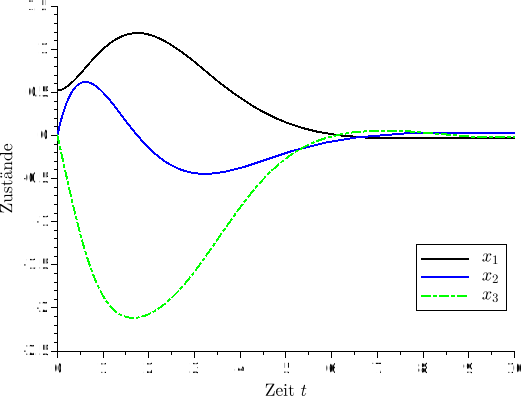
\includegraphics[width=0.8\textwidth]{Inv_Pendel_Motor_LQR}
\par\end{centering}
\caption{Einschwingverhalten des durch LQR-Entwurf in den transformierten Koordinaten
geregelten Pendels\label{fig:opt-inv-pendel-motor-lqr}}

\end{figure}
\end{example}

\subsection{Sontag-Formel}

Die Optimalität des im vorangegangenen Abschnitt hergeleiteten Regelgesetzes~(\ref{eq:opt-LQR-EZ-lin})
hinsichtlich eines quadratischen Gütekriteriums bezieht sich allerdings
nicht auf das Originalsystem~(\ref{eq:basissystem-optimierung}),
sondern auf das transformierte und durch die Rückführung linearisierte
System~(\ref{eq:opt-linearisiertes-system}). In den Originalkoordinaten
ist das Regelgesetz~(\ref{eq:opt-LQR-EZ-lin}) in der Regel keine
Lösung eines Optimierungsproblems\footnote{Die Aussage, dass das Regelgesetz~(\ref{eq:opt-LQR-EZ-lin}) in der
Regel nicht optimal im Sinne eines Kostenfunktionals~(\ref{eq:opt-Kosten-nl})
ist, lässt dadurch veranschaulichen, dass die Rückführung~(\ref{eq:opt-LQR-EZ-lin})
alle im System auftretenden Nichtlinearitäten kompensiert, auch jene,
die die Stabilität begünstigen.} mit einem Kostenfunktional der Form~(\ref{eq:opt-Kosten-nl}). In
diesem Abschnitt wird ein Regelgesetz angegeben, welches das System~(\ref{eq:basissystem-optimierung})
stabilisiert und zugleich Lösung eines Optimierungsproblems ist. Dieser
Zugang ist unter der Bezeichnung \emph{invers-optimale}\index{invers-optimale Regelung}
oder \emph{modifizierte optimale Regelung} \index{modifizierte optimale Regelung}
bekannt~\cite{freeman96control,freeman96siam,freeman1996buch,sepulchre97,sackmann2005modifizierte}.

Zunächst verallgemeinern wir den Begriff der Ljapunov-Funktion auf
Systeme mit Erregung. Sei $V:\R^{n}\to\R$ eine stetig differenzierbare,
positiv definite Funktion (siehe Anhang~\ref{sec:Stabilitaet-autonomer-Systeme}).
Die Funktion~$V$ nennt man \emph{Regelungs-Ljapunov-Funktion}\index{Regelungs-Ljapunov-Funktion}
(engl. \emph{control Lyapunov function}, kurz \emph{CLF}) von System~(\ref{eq:basissystem-optimierung}),
falls
\begin{equation}
\forall x\neq0:\quad\inf_{u}\left(L_{f}V(x)+L_{g}V(x)u\right)<0.\label{eq:CLF-def1}
\end{equation}
Mit der Existenz einer Regelungs-Ljapunov-Funktion gibt es auch eine
stabilisierende Zustandsrückführung~\cite{artstein1983}:
\begin{theorem}
[Theorem von Artstein]\label{thm:Artstein}Man betrachte das System~(\ref{eq:basissystem-optimierung})
mit $f(0)=0$. Ferner sei~$V$ eine Regelungs-Ljapunov-Funktion.
Dann gibt es eine Zustandsrückführung~(\ref{eq:opt-kappa}) derart,
dass $x=0$ eine asymptotisch stabile Ruhelage des geschlossenen Regelkreises
ist.
\end{theorem}
\begin{proofsketch}Sie~$V$ eine Regelungs-Ljapunov-Funktion von
System~(\ref{eq:basissystem-optimierung}). Die Zeitableitung von~$V$
entlang der Systemdynamik von~(\ref{eq:basissystem-optimierung})
hat die Form
\begin{equation}
\begin{array}{ccl}
\dot{V}(x) & = & V^{\prime}(x)\cdot\dot{x}\\
 & = & V^{\prime}(x)\cdot f(x)+g(x)u\\
 & = & L_{f}V(x)+L_{g}V(x)u.
\end{array}\label{eq:opt-Vdot1}
\end{equation}
Bedingung~(\ref{eq:CLF-def1}) bedeutet, dass man den Eingang~$u$
in Abhängigkeit vom Zustand~$x$ immer so wählen kann, dass~$\dot{V}$
negativ definit ist. Damit ist~$V$ eine Ljapunov-Funktion des in
dieser Weise rückgeführten Systems und die Ruhelage $x=0$ ist asymptotisch
stabil.\end{proofsketch}

Die Bedingung~(\ref{eq:CLF-def1}) ist gleichwertig mit 
\begin{equation}
L_{g}V(x)=0\quad\Longrightarrow\quad L_{f}V(x)<0.\label{eq:CLF-def2}
\end{equation}
In den Punkten~$x$, wo die Ableitung~$\dot{V}$ wegen $L_{g}V(x)=0$
nicht über den Eingang~$u$ beeinflusst werden kann, muss das Vektorfeld~$f$
einen Beitrag zur Stabilität liefern.

Kennt man zu einem gegebenen System~(\ref{eq:basissystem-optimierung})
eine Regelungs-Lyapunov-Funktion~$V$, dann stellt die \emph{Sontag-Formel}\index{Sontag-Formel}~\cite{sontag89,sontag98}
\begin{equation}
u=-\kappa(x)=\left\{ \begin{array}{ccc}
-\frac{L_{f}V(x)+\sqrt{\left[L_{f}V(x)\right]^{2}+\left[L_{g}V(x)\right]^{4}}}{L_{g}V(x)} & \text{falls} & L_{g}V(x)\neq0\\
0 & \text{falls} & L_{g}V(x)=0
\end{array}\right.\label{eq:sontag-formel}
\end{equation}
eine stabilisierende Zustandsrückführung~(\ref{eq:opt-kappa}) bereit.
Setzt man~(\ref{eq:sontag-formel}) in das System ein, dann ergibt
sich aus~(\ref{eq:opt-Vdot1}) die Zeitableitung
\[
\dot{V}(x)=\left\{ \begin{array}{ccc}
-\sqrt{\left[L_{f}V(x)\right]^{2}+\left[L_{g}V(x)\right]^{4}} & \text{falls} & L_{g}V(x)\neq0,\\
L_{f}V(x) & \text{falls} & L_{g}V(x)=0.
\end{array}\right.
\]
Dadurch ist~$\dot{V}$ negativ definit und die Ruhelage $x=0$ des
geschlossenen Regelkreis asymptotisch stabil.

Mit der Rückführung~(\ref{eq:sontag-formel}) stabilisiert man nicht
nur das System~(\ref{eq:basissystem-optimierung}), sondern minimiert
auch ein Kostenfunktional~(\ref{eq:opt-Kosten-nl}). Stellt man die
Rückführung~(\ref{eq:opt-LgV-Regelgesetz}) nach der Wichtungsfunktion~$p$
um, so erhält man 
\begin{equation}
p(x)=\frac{1}{2\kappa(x)}\,L_{g}V(x).\label{eq:inv-opt-p}
\end{equation}
Durch Einsetzen dieser Funktion in die Hamilton-Jacobi-Bellman-Gleichung~(\ref{eq:HJB})
bekommt man die zweite Wichtungsfunktion:
\begin{equation}
q(x)=\frac{1}{4p(x)}\left(L_{g}V(x)\right)^{2}-L_{f}V(x).\label{eq:inv-opt-q}
\end{equation}
Damit ist~(\ref{eq:sontag-formel}) die Lösung des durch das Kostenfunktional~(\ref{eq:opt-Kosten-nl})
mit~(\ref{eq:inv-opt-p}) und~(\ref{eq:inv-opt-q}) beschriebenen
Optimierungsproblems. Die zur Stabiliserung herangezogene Regelungs-Ljapunov-Funktion~$V$
ist dann auch die zugehörige Bellman-Funktion. Die unterschiedlichen
Herangehensweisen bei der optimalen bzw. der invers-optimalen Regelung
werden im nachfolgenden Diagramm veranschaulicht:

\[
\begin{CD}
\text{Kostenfunktional} @. \text{Kostenfunktional}\\
@V{\text{Gl.~\eqref{eq:HJB}}}VV @ AA{\text{Gln.~\eqref{eq:inv-opt-p}, \eqref{eq:inv-opt-q}}}A\\
\text{Bellman-Funktion}~V @= \text{Regelungs-Ljapunov-Funktion}~V\\
@V{\text{Gl.~\eqref{eq:opt-LgV-Regelgesetz}}}VV @VV{\text{Gl.~\eqref{eq:sontag-formel}}}V\\
\text{Regelgesetz} @. \text{Regelgesetz}
\end{CD}
\]

Eine wichtige Konsequenz aus der Optimalität der Zustandsrückführung~(\ref{eq:sontag-formel})
ist die Robustheit des so geregelten System~\cite{freeman96control,freeman96siam,sepulchre97}.
Von der Sontag-Formel~(\ref{eq:sontag-formel}) wurden auch zahlreiche
Abwandlungen entwickelt bzw. erprobt~\cite{lin1991,malisoff2000scl,yu2001}.

\medskip{}

In der Regel ist es sehr schwierig, für ein gegebenes System eine
Regelungs-Ljapunov-Funktion zu finden. Ist das System~(\ref{eq:basissystem-optimierung})
eingangs-zustands-linearisierbar, dann kann es durch die Rückführung~(\ref{eq:opt-rueck-linearisierend})
in das lineare System~(\ref{eq:opt-linearisiertes-system}) überführt
werden. Zu diesem System berechnet man für eine gegebene Matrix $Q\succeq0$
und eine Zahl $R>0$ eine positiv definite Lösung $P\succ0$ der algebraischen
Riccati-Gleichung~(\ref{eq:var-opt-ARE}). Damit erhält man in den
transformierten Koordinaten die Bellman-Funktion $\widetilde{V}(\xi)=\xi^{T}P\xi$.
Diese ist zugleich eine Regelungs-Ljapunov-Funktion des linearisierten
Systems~(\ref{eq:opt-linearisiertes-system}), denn über die Rückführung
$v=-k^{T}\xi$ mit~(\ref{eq:var-opt-k}) erhält man eine asymptotisch
stabile Ruhelage $\xi=0$. Daraus ergibt sich in Originalkoordinaten
die Regelungs-Ljapunov-Funktion
\begin{equation}
V(x)=\widetilde{V}(\Phi(x))=\Phi^{T}(x)\,P\,\Phi(x).\label{eq:inv-opt-CLF-EZ}
\end{equation}
Mit der durch die Sontag-Formel~(\ref{eq:sontag-formel}) gegebenen
Rückführung erhält man ein robustes Regelgesetz. 

Bei einem gegebenen System~(\ref{eq:basissystem-optimierung}) lässt
sich das Vorgehen zum Entwurf der beschriebenen invers-optimalen Regelung
folgendermaßen zusammenfassen:
\begin{enumerate}
\item Bestimmung einer Ausgangsabbildung~$h$, für die das System~(\ref{eq:basissystem-optimierung})
den relativen Grad~$n$ besitzt (siehe Abschnitt~\ref{sec:Exakte-Eingangs-Zustands-Linearisierung}).
\item Berechnung der Lie-Ableitungen $L_{f}h(x),\ldots L_{f}^{n-1}h(x)$. 
\item Berechnung einer positiv definiten Lösung~$P$ der algebraischen
Riccati-Gl.~(\ref{eq:var-opt-ARE}) für das linearisierte System~(\ref{eq:opt-linearisiertes-system}),
z.\,B. mit $Q=I$ und $R=1$.
\item Berechnung der Regelungs-Ljapunov-Funktion~(\ref{eq:inv-opt-CLF-EZ})
mit $\xi_{1}=h(x),\ldots,\xi_{n}=L_{f}^{n-1}h(x)$.
\item Berechnung der Lie-Ableitungen $L_{f}V(x)$ und $L_{g}V(x)$.
\item Berechnung der Zustandsrückführung~(\ref{eq:sontag-formel}).
\end{enumerate}

Die Vorgehensweise zur Nutzung der Sontag-Formel~(\ref{eq:sontag-formel})
für eingangs-zustands-linearisierbare Systeme wird an einem Beispiel
vorgestellt:

\begin{example}
Wir betrachten das bereits in Beispiel~\ref{exa:Inverses-Pendel-Motor-LQR}
behandelte inverse Pendel mit Gleichstrommotor. Aus~(\ref{eq:opt-inv-pendel-motor-lie})
liest man die Koordinatentransformation 
\[
\Phi(x)=\left(\begin{array}{c}
h(x)\\
L_{f}h(x)\\
L_{f}^{2}h(x)
\end{array}\right)=\left(\begin{array}{c}
x_{1}\\
x_{2}\\
\frac{-d{\it x_{2}}+mg\ell\sin{\it x_{1}}+K{\it x_{3}}}{J}
\end{array}\right)
\]
ab. Zusammen mit der Matrix~$P$ aus Gl.~(\ref{eq:opt-inv-pendel-motor-P})
erhält man die Regelungs-Ljapunov-Funktion~(\ref{eq:inv-opt-CLF-EZ}),
mit deren Hilfe man die Zustandsrückführung~(\ref{eq:sontag-formel})
angeben kann. Zu Beginn der Simulation wird die Zustandskomponente~$x_{3}$
sehr stark beeinflusst, so dass sie fast unmitelbar von $x_{3}(0)=0$
auf den Wert von ca. $1,09$ übergeht. Bezogen auf die eigentliche
Regelgröße~$x_{1}$ ist im Unterschied zu Beispiel~\ref{exa:Inverses-Pendel-Motor-LQR}
kein Überschwingen zu erkennen.

\begin{figure}
\begin{centering}
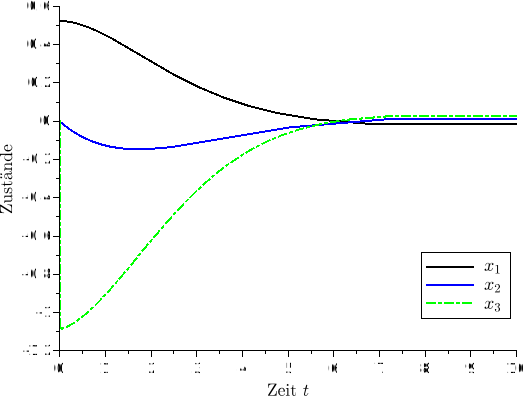
\includegraphics[width=0.8\textwidth]{Inv_Pendel_Motor_Sontag}
\par\end{centering}
\caption{Einschwingverhalten des mit Hilfe der Sontag-Formel geregelten Pendels\label{fig:opt-inv-pendel-motor-sontag}}
\end{figure}
\end{example}
\bibliographystyle{babalpha}
\bibliography{dynamic}

